\documentclass[10pt,landscape,a4paper]{article}
\usepackage[utf8]{inputenc}
\usepackage[ngerman]{babel}
\usepackage{tikz}
\usetikzlibrary{shapes,positioning,arrows,fit,calc,graphs,graphs.standard}
\usepackage[nosf]{kpfonts}
\usepackage[t1]{sourcesanspro}
%\usepackage[lf]{MyriadPro}
%\usepackage[lf,minionint]{MinionPro}
\usepackage{multicol}
\usepackage{wrapfig}
\usepackage[top=5mm,bottom=5mm,left=5mm,right=5mm]{geometry}
\usepackage[framemethod=tikz]{mdframed}
\usepackage{microtype}
\usepackage{bbold}
\usepackage{wrapfig}
\usepackage{dsfont} % For mathbb{1}
\usepackage{amsmath}

% START CHEATSHEET TEMPLATE

\usepackage[default]{raleway}
\usepackage{fontawesome}
\usepackage[T1]{fontenc}

\usepackage{hyperref}
\usepackage{enumitem}
\setlist[enumerate]{itemsep=0mm}
\usepackage{lipsum}

\usepackage{xcolor}
\definecolor{customcolor}{HTML}{b5e9ff}
\definecolor{alert}{HTML}{CD5C5C}
\definecolor{w3schools}{HTML}{4CAF50}
\definecolor{subbox}{gray}{0.60}
\definecolor{codecolor}{HTML}{000000}
\colorlet{xx}{customcolor}

\usepackage{paralist}


%--------------------------Editor mode.

\usepackage
[citestyle=authoryear,
sorting=nty,	  		%Sorts bibliography by year, name, title
autocite=footnote, 		%Autocite command generates footnotes
autolang=hyphen, 		
mincrossrefs=1, 	
backend=biber]
{biblatex}

\DeclareFieldFormat{postnote}{#1}
\DeclareFieldFormat{multipostnote}{#1}
\DeclareAutoCiteCommand{footnote}[f]{\footcite}{\footcites}

\bibliography{literature}
%----------------------------------------
%--------------------------------------------------------------------------------
\usepackage{tcolorbox}

\tcbuselibrary{most,listingsutf8,minted}

\tcbset{tcbox width=auto,left=1mm,top=1mm,bottom=1mm,
right=1mm,boxsep=1mm,middle=1pt}

\newenvironment{mycolorbox}[2]{%
\begin{tcolorbox}[grow to left by=-1em,grow to right by=-1em,capture=minipage,fonttitle=\large\bfseries, enhanced jigsaw,boxsep=1mm,colback=#1!30!white,on line,tcbox width=auto, toptitle=0mm,colframe=#1,opacityback=0.7,nobeforeafter,title=#2]%
}{\end{tcolorbox}\\[0.2em]}

\newenvironment{subbox}[2]{%
\begin{tcolorbox}[capture=minipage,fonttitle=\normalsize\bfseries, enhanced jigsaw,boxsep=1mm,colback=#1!30!white,on line,tcbox width=auto,left=0.3em,top=1mm, toptitle=0mm,colframe=#1,opacityback=0.7,nobeforeafter,title=#2]\footnotesize %
}{\normalsize\end{tcolorbox}\vspace{0.1em}}

\newenvironment{multibox}[1]{%
\begin{tcbraster}[raster columns=#1,raster equal height,nobeforeafter,raster column skip=1em,raster left skip=1em,raster right skip=1em]}{\end{tcbraster}}

\newenvironment{textbox}[1]{\begin{mycolorbox}{customcolor}{#1}}{\end{mycolorbox}}

%-------------------------------
\newtcblisting{codebox}[2]{colback=codecolor!5,colframe=codecolor!80!black,listing only, 
minted options={numbers=left,style=tcblatex,fontsize=\scriptsize,breaklines,autogobble,linenos=false,numbersep=2mm},
left=4mm,enhanced,boxsep=1pt,left=2pt,right=1pt,top=0pt,bottom=0pt,
title=#2, fonttitle=\bfseries,
listing engine=minted,minted language=#1}

%--------------------------------------------------------------------------------
\newcommand{\punkti}{~\lbrack\dots\rbrack~}

\renewenvironment{quote}
               {\list{\faQuoteLeft\phantom{ }}{\rightmargin\leftmargin}%
                \item\relax\scriptsize\ignorespaces}
               {\unskip\unskip\phantom{xx}\faQuoteRight\endlist}
               

%--------------------------------------------------------------------------------
\newcommand{\bgupper}[3]{\colorbox{#1}{\color{#2}\huge\bfseries\MakeUppercase{#3}}}
\newcommand{\bg}[3]{\colorbox{#1}{\bfseries\color{#2}#3}}

\newcommand{\mycommand}[2]{{\ttfamily\detokenize{#1}}~\dotfill{}~{\footnotesize #2}\\}
\newcommand{\sep}{{\scriptsize~\faCircle{ }~}}


\newcommand{\bggreen}[1]{\medskip\bgupper{w3schools}{black}{#1}\\[0.5em]}
\newcommand{\green}[1]{\smallskip\bg{w3schools}{white}{#1}\\}
\newcommand{\red}[1]{\smallskip\bg{alert}{white}{#1}\\}

\usepackage{multicol}
\setlength{\columnsep}{4pt}

\setlength{\parindent}{0pt}
\pagestyle{empty}

\usepackage{csquotes}

\newcommand{\loremipsum}{Lorem ipsum dolor sit amet.}

% END CHEATSHEET TEMPLATE

\let\bar\overline

\definecolor{myblue}{cmyk}{1,.72,0,.38}

\def\firstcircle{(0,0) circle (1.5cm)}
\def\secondcircle{(0:2cm) circle (1.5cm)}

\colorlet{circle edge}{myblue}
\colorlet{circle area}{myblue!5}

\tikzset{filled/.style={fill=circle area, draw=circle edge, thick},
    outline/.style={draw=circle edge, thick}}

\pgfdeclarelayer{background}
\pgfsetlayers{background,main}

\everymath\expandafter{\the\everymath \color{myblue}}
\everydisplay\expandafter{\the\everydisplay \color{myblue}}

\renewcommand{\baselinestretch}{.8}
\pagestyle{empty}




\makeatletter
\renewcommand{\section}{\@startsection{section}{1}{0mm}%
                                {.2ex}%
                                {.2ex}%x
                                {\color{myblue}\sffamily\small\bfseries}}
\renewcommand{\subsection}{\@startsection{subsection}{1}{0mm}%
                                {.2ex}%
                                {.2ex}%x
                                {\sffamily\bfseries}}
\makeatother

\def\multi@column@out{%
   \ifnum\outputpenalty <-\@M
   \speci@ls \else
   \ifvoid\colbreak@box\else
     \mult@info\@ne{Re-adding forced
               break(s) for splitting}%
     \setbox\@cclv\vbox{%
        \unvbox\colbreak@box
        \penalty-\@Mv\unvbox\@cclv}%
   \fi
   \splittopskip\topskip
   \splitmaxdepth\maxdepth
   \dimen@\@colroom
   \divide\skip\footins\col@number
   \ifvoid\footins \else
      \leave@mult@footins
   \fi
   \let\ifshr@kingsaved\ifshr@king
   \ifvbox \@kludgeins
     \advance \dimen@ -\ht\@kludgeins
     \ifdim \wd\@kludgeins>\z@
        \shr@nkingtrue
     \fi
   \fi
   \process@cols\mult@gfirstbox{%
%%%%% START CHANGE
\ifnum\count@=\numexpr\mult@rightbox+2\relax
          \setbox\count@\vsplit\@cclv to \dimexpr \dimen@-1cm\relax
\setbox\count@\vbox to \dimen@{\vbox to 1cm{\header}\unvbox\count@\vss}%
\else
      \setbox\count@\vsplit\@cclv to \dimen@
\fi
%%%%% END CHANGE
            \set@keptmarks
            \setbox\count@
                 \vbox to\dimen@
                  {\unvbox\count@
                   \remove@discardable@items
                   \ifshr@nking\vfill\fi}%
           }%
   \setbox\mult@rightbox
       \vsplit\@cclv to\dimen@
   \set@keptmarks
   \setbox\mult@rightbox\vbox to\dimen@
          {\unvbox\mult@rightbox
           \remove@discardable@items
           \ifshr@nking\vfill\fi}%
   \let\ifshr@king\ifshr@kingsaved
   \ifvoid\@cclv \else
       \unvbox\@cclv
       \ifnum\outputpenalty=\@M
       \else
          \penalty\outputpenalty
       \fi
       \ifvoid\footins\else
         \PackageWarning{multicol}%
          {I moved some lines to
           the next page.\MessageBreak
           Footnotes on page
           \thepage\space might be wrong}%
       \fi
       \ifnum \c@tracingmulticols>\thr@@
                    \hrule\allowbreak \fi
   \fi
   \ifx\@empty\kept@firstmark
      \let\firstmark\kept@topmark
      \let\botmark\kept@topmark
   \else
      \let\firstmark\kept@firstmark
      \let\botmark\kept@botmark
   \fi
   \let\topmark\kept@topmark
   \mult@info\tw@
        {Use kept top mark:\MessageBreak
          \meaning\kept@topmark
         \MessageBreak
         Use kept first mark:\MessageBreak
          \meaning\kept@firstmark
        \MessageBreak
         Use kept bot mark:\MessageBreak
          \meaning\kept@botmark
        \MessageBreak
         Produce first mark:\MessageBreak
          \meaning\firstmark
        \MessageBreak
        Produce bot mark:\MessageBreak
          \meaning\botmark
         \@gobbletwo}%
   \setbox\@cclv\vbox{\unvbox\partial@page
                      \page@sofar}%
   \@makecol\@outputpage
     \global\let\kept@topmark\botmark
     \global\let\kept@firstmark\@empty
     \global\let\kept@botmark\@empty
     \mult@info\tw@
        {(Re)Init top mark:\MessageBreak
         \meaning\kept@topmark
         \@gobbletwo}%
   \global\@colroom\@colht
   \global \@mparbottom \z@
   \process@deferreds
   \@whilesw\if@fcolmade\fi{\@outputpage
      \global\@colroom\@colht
      \process@deferreds}%
   \mult@info\@ne
     {Colroom:\MessageBreak
      \the\@colht\space
              after float space removed
              = \the\@colroom \@gobble}%
    \set@mult@vsize \global
  \fi}

\makeatother
\setlength{\parindent}{0pt}

\begin{document}
\begin{multicols*}{4}
\scriptsize
\section*{Background}
$\log(x+1)\approx x$ if $|x|<<1$ \\
\textbf{Variance and covariance:}\\
$\mathbb{V}\text{ar}(X) = \text{Cov}(X,X) = \mathbb{E}[ (X - \mathbb{E}X)^2] = \mathbb{E}[X^2] - (\mathbb{E}[X])^2$ \\
$\text{Cov}(\mathbf X, \mathbf Y)=\mathbb E[(\mathbf X - \mathbb E\mathbf X)(\mathbf Y - \mathbb E\mathbf Y)^T]=\mathbb E[\mathbf{XY}^T]-\mathbb E[\mathbf X]\mathbb E[\mathbf Y]^T$\\
$\text{Cov}(aX+bY,cW+dV)=ac\text{Cov}(X,W)+ad\text{Cov}(X,V)+bc\text{Cov}(Y,W)+bd\text{Cov}(Y,V)$\\
\textbf{Integration by parts}: $\int f \cdot g' = f\cdot g - \int f' \cdot g$\\
\textbf{Geometric sums \& series:} $\sum_{k=0}^nar^k=a(\frac{1-r^{n+1}}{1-r})\overset{n\rightarrow\infty}{\longrightarrow}\frac{a}{1-r}, |r|<1$\\
\textbf{Hoeffding's inequality: }\\ For $Z_i \in [0,1]$ iid, 
$\mathbb P(\frac{1}{n}\sum_{i=1}^n Z_i - \mathbb E[Z]\geq t)\leq\exp\{-2n t^2\}$. \\
For $Z_i \in [a_i,b_i]$ the upper bound is $\exp(-\frac{2nt^2}{\sum_{i=1}^n(b_i -a_i)^2})$\\
\textbf{Boole's inequality - union bound} $\mathbb{P}\left(\underset{i}{\bigcup} A_i \right) \leq \underset{i}{\sum} \mathbb{P}(A_i)$ \\
\textbf{Cauchy-Schwarz inequality}: $v^Tu\leq||v||_2||u||_2$\\
\textbf{Hölder's inequality}: $v^Tu\leq ||v^Tu||_1\leq||v||_{p}||u||_{p^*}$, \\ where $1/p+1/p^*=1$, equality if $|v|^p=\gamma|u|^{p^*}$\\
\textbf{Jensen's inequality}: $f$ convex, then $f(\mathrm E[X])\leq\mathrm E[f(X)]$\\
$\Rightarrow \log(\mathrm E[X])\geq\mathrm E[\log(X)]$ \\
\textbf{Markov's inequality:} $\mathrm P(X\geq a)\leq\frac{\mathrm E[X]}{a}$\\
\textbf{KL Divergence} Let $Q$, $P$ be prob. distr. of a continuous RV $x \in \mathbb{R}^d$, with densities $q$,$p$. Then  $KL(Q || P) = \int_{-\infty}^{\infty} q(x)\log \frac{q(x)}{p(x)}dx$\\
\textbf{Entropy} For $X \in \{x_1,..,x_n \}$, $H(X) = - \sum P(x_i)\log P(x_i) $

$\left( \underset{i}{\sum}a_i\right)^2 = \underset{i}{\sum}a_i^2 + 2\underset{i<j}{\sum}a_ia_j$\\
For square matrices $A$, $B$: $\det A = \det A^t$, $\det AB = \det A \cdot \det B$, $\det A^{-1} = \frac{1}{\det A }$\\
\textbf{Moment Generating Function}
$M_x :\mathbb{R}^n \rightarrow \mathbb{R}$, $M_x(t) = \mathbb{E}_x[\exp(t\cdot x)]$. $M_{x+y} = M_x\cdot M_y$\\
For $x \sim \mathcal{N}(\mu, \Sigma)$, we have $M_x(t) = \exp(t\cdot\mu + \frac{1}{2}t^T\Sigma t$
%%%% LOSSES %%%%
\subsection*{Losses}
%Assume classification problem with $M$ classes. \\
Cross entropy loss $H(x) = -\overset{M}{\underset{c=1}{\sum}} y_{o,c}\log P(x_{o,c})$ \\

%%%% DISTRIBUTIONS %%%%

\subsection*{Distributions}
\textbf{Standard normal}: $p(x|\mu, \sigma^2)=\frac{e^{-(x-\mu)^2/(2\sigma^2)}}{\sqrt{2\pi\sigma^2}}$\\
\textbf{Multivariate normal:} $x \sim \mathcal{N}(\mu, \Sigma)$\\
$p(x|\mu, \Sigma) = \frac{1}{(2\pi)^\frac{k}{2}\det(\Sigma)^{\frac{1}{2}}} \exp(-\frac{1}{2}(x-\mu)^t\Sigma^{-1}(x-\mu))$\\
\textbf{Exponential:} $p(x|\lambda)=\lambda e^{-\lambda x}$\\
\textbf{Bernoulli:} $p(x|p)=p^x (1-p)^{1-x}$\\
\textbf{Binomial:} $p(x|n,p)={n\choose x}p^x (1-p)^{n-x}$\\
\textbf{Poisson:} $p(x|\lambda)=\frac{\lambda^x\exp[-\lambda]}{x!}$
\section*{Connectionism}
\textbf{McCulloch \& Pitts neuron:} $f(x;\mathbf{\sigma,\theta})=\begin{cases} 
       1, \quad \sum_{i=1}^n\sigma_i x_i\geq\theta\\
       0, \quad \text{else}
       \end{cases}$ \\
$x\in\{0,1\}^n, \quad \sigma\in\{\pm 1\}^n, \quad \theta\in\mathbb{Z}$\\
Disjunctive Normal Form: $f(\mathbf{x};\sigma,\theta)=\bigvee_{I\in\mathcal{I}}(\bigwedge_{i\in I}x_i\bigwedge_{i\notin I}\bar x_i),$\\
$\mathcal{I}=\{I: \sum_{i\in I}\sigma_i\geq \theta\}$ (OR of ANDs)\\
\textbf{Turing Type A machine (NAND):}\\ $y(t+1)=1-x_1(t)x_2(t), \quad x_1(t),x_2(t)\in\{0,1\}$\\
\textbf{Turing Type B machine:}\\
$A(1,\text{NAND}(x_1,x_1))=x_1, \quad A(0,\text{NAND}(x_1,x_1))=1$\\
$\text{NAND}(A,x_2,...,x_n)=\begin{cases} \text{NAND}(x_2,...,x_n) \quad \text{if } A\leftarrow 1 \\ \text{NAND}(x_1,...,x_n) \quad \text{else}\end{cases}$

\subsection*{Perceptron}
$(\mathbf{x,\theta})\rightarrow \text{sgn}(\mathbf{x\cdot\theta}),\quad$  update rule: $\Delta\mathbf{\theta}=\begin{cases} 
       \mathbf{0}, \quad y(\mathbf{x\cdot\theta})\geq 0\\
       y\mathbf x, \quad \text{otherwise}
       \end{cases}$\\
Path of updates always zig-zag since $\Delta\mathbf{\theta\cdot\theta}<0$ for updates \\
Update rule is SGD for the loss: $l(\mathbf x,y;\mathbf\theta)=\max\{0,-y\mathbf{x\cdot\theta}\}$\\
\textbf{Lemma (Norm Growth)}: $(\mathbf x^t, y^t)$ perceptron mistakes inducing updates $\Delta\mathbf\theta^t, \mathbf\theta^s=\sum_{t=1}^s\Delta\mathbf\theta^t$. Then:\\
$||\mathbf\theta^s||^2\leq\sum_{t=1}^s||\mathbf x^t||^2 \quad$ (prove by induction!)\\
\textbf{Cor: } If $||\mathbf x^t||\leq 1$ then $||\mathbf\theta^s||\leq\sqrt s$\\
\textbf{Def (Linear Separability)}:  $\mathcal{S}$ linearly separable with margin $\gamma>0$ if $\exists \mathbf\theta^*, ||\mathbf\theta^*||=1:y\mathbf{x\cdot\theta^*}\geq\gamma>0 \quad \forall(\mathbf x, y)\in\mathcal S$\\
\textbf{Novikov's convergence theorem:} Converges in at most $\gamma^{-2}$ steps (if assume $||\mathbf x^t||\leq 1$). Show $\gamma s\leq s$ and start with fact that $\Delta\theta^t\theta^* = y^tx^t\theta^*\geq \gamma$ $+$ $\theta^s=\sum\Delta\theta^t$ $+$ Cauchy-Schwarz\\
\textbf{Cover's theorem}: Dichotomies possible with linear separators: $C(s,n)=2\sum_{i=0}^{n-1} {s-1\choose i}$\\
Prove by showing recurrence relation $C(s+1,n)=C(s,n)+C(s,n-1)$ using Pascal's rule: ${n-1 \choose k} + {n-1 \choose k-1}={n \choose k}$\\
\textbf{VC dimension:} largest set $S$ that can be shattered. Corollary of Cover's thm: $n$ points can be shattered by linear functions in $n$ dimensions (meaning can realize all $2^n$ points). $m>n$ can not.
\subsection*{Willshaw Memory}
\textbf{Hebb rule}: $\Delta\theta_{ij}^t\propto x_i^tx_j^t$ (neurons that fire together, wire together)\\
\textbf{r-sparse Boolean vectors} $\mathbb{B}_r^n=\{x\in\{0,1\}^n|\sum x_i \leq r\}$\\
\textbf{Upper bound on number of patterns $s$:} $s\leq\frac{n^2}{r\log n}, \\ \log {n\choose r}\approx r\log n$ is pattern information and $n^2$ total number of bits\\
\textbf{Binary memory matrix:} $\Theta_{ji} = \min\{1,\sum_{t=1}^sy_j^tx_i^t\}$, $\Theta_{ji} \in \{0,1\}^{nxn}$ \\ Alternatively: $\Theta=\min\{\mathbf 1,\sum_{t=1}^s\mathbf y^t(\mathbf x^t)^T\}$\\
\textbf{Retrieve $y$ from given $x$:} $z=\Theta x, \quad y_j=\begin{cases} 0 \quad z_j<r \\ 1 \quad \text{else} \end{cases}$\\
\textbf{Monotonicity:} $x^t\mapsto y\geq y^t, \forall (x^t,y^t)\in\mathcal S$ (i.e. get at least as much as ask for). Proof: $\Theta=\min\{\mathbf 1,\sum_{\tau}\Theta^\tau\}\geq\min\{\mathbf 1,\Theta^t\}=\Theta^t$\\
$\mathbf z^t=\Theta \mathbf x^t\geq\Theta^t \mathbf x^t=\mathbf y^t(\mathbf x^t)^T\mathbf x^t=r\mathbf y^t$\\
\textbf{Maximal capacity:} $\max_qI(\text{patterns})=(\log 2)n^2\approx 0.693n^2$ in the limit, for $r=\log n$. Half of $\theta_{ji}$ will be $0$ and half will be $1$ as $n\rightarrow\infty$
\subsection*{Hopfield Networks}
\textbf{Idea:} Store patterns in $\Theta$, for recovery from corrupted patterns\\
$\Theta=\sum_{t=1}^s[x_tx_t^T-\mathrm I_n]\in\mathrm Z^{n\times n}$\\
Asynchronous update: $\tilde x_i\leftarrow \text{sign}(\sum_{j\neq i}\theta_{ij}\tilde x_j+\theta_{i0})$  (Hopfield dynamics)\\
Synchronous updates can lead to limit cycles\\
Lyapunov function: $\Epsilon=-\sum_{i,j=1}^n\theta_{ij}x_ix_j-\sum_{i=1}^n\theta_{i0}x_i$\\
\textbf{Hebb -Hopfield} $\Theta \approx \underset{t=1}{\overset{s}{\sum}}[x^{t}^Tx^t-I]$ $\in \mathbb{R}^{nxn}$. Use fact that for $\hat{x}$ with hamming-dist $k$ to $x$, $x\cdot\hat{x}-1 = (n-2k-1)$ to show $-x,x$ both attractors. Capacity for num of patterns is $\frac{\alpha}{n} \leq \alpha^* \approx 0.138$. For Hopfield (without Hebb's rule, but with optimal weights) $\alpha^* = 2$
\section*{Linear Networks}
Linear unit: $\iota(\mathbf x;\pmb\theta)=\mathbf x\cdot \pmb\theta,\quad$ Affine unit: $\iota(\mathbf x;\pmb\theta,b)=\mathbf x\cdot \pmb\theta+b$\\
Level sets: $\iota(\mathbf x +\Delta\mathbf x,\mathbf \theta)=\iota(\mathbf x, \mathbf \theta), \quad \Delta\mathbf x\perp \mathbf \theta$\\
Linear unit defines: direction of change via $\mathbf{\frac{\theta}{||\theta||}}$, rate of change via $||\mathbf \theta||$\\
Learning algo for linear units: $\Delta\mathbf\theta=\eta(y-\mathbf{x\cdot\theta)x}$\\
Homogeneity: $f(\alpha \mathbf x)=\alpha f(\mathbf x)$\\
Additivity: $f(\mathbf{x+y})=f(\mathbf x)+f(\mathbf y)$\\
$\Rightarrow f$ is linear with these properties\\
$f, g$ linear $\Rightarrow f\circ g$ linear\\
Affine functions: $f(\alpha\mathbf x+\beta\mathbf y)=\alpha f(\mathbf x)+\beta f(\mathbf y), \quad \forall\mathbf{x,y}:\forall \alpha,\beta: \alpha+\beta = 1$
\subsection*{Linear Autoencoder}
Def: $\mathbf{x\mapsto z \mapsto y}, \quad \mathbf{z=Cx, y=Dz, \quad C,D}^T\in\mathbb R^{m\times n}, m<n$\\
Loss: $l(\mathbf x)=\frac{1}{2}||\mathbf{x-y}||^2$\\
Matrix notation: $\mathbf{X,Y}\in\mathbb{R}^{n\times s}:\quad \mathbf{\theta=(C,D)}\rightarrow_{min}\frac{1}{2s}||\mathbf{X-DCX}||^2_F$\\
$\frac{\delta l(\mathbf x)}{\delta\mathbf C}=\mathbf D^T(\mathbf{y-x})\mathbf x^T\in\mathbb R^{m\times n}$\\
$\frac{\delta l(\mathbf x)}{\delta\mathbf D}=\mathbf{(y-x)x}^T\mathbf C^T\in\mathbb{R}^{n\times m}$\\
$\text{rank}(\mathbf{DC})\leq\min\{\text{rank}(\mathbf C), \text{rank}(\mathbf D)\}\leq m<n \quad\Rightarrow  \text{rank}(\mathbf{Y})\leq m$\\
\textbf{Eckhart-Young Theorem: } $||\mathbf{X-X}_r||_F=\min_{\text{rank}(\mathbf Y)\leq r}||\mathbf{X-Y}||_F$\\
$\mathbf{C=U}_m^T, \mathbf{D=U}_m \Rightarrow \mathbf{DCX=X}_m$
\subsection*{Gradients of deep linear networks}
Assume $\mathbf{X,Y}$ centered, $\mathbf X$ whitened: $\mathbf X\mapsto \mathbf{\Lambda}^{-\frac{1}{2}}\mathbf U^T\mathbf X, \text{s.t.} \frac{1}{s}\mathbf{XX}^T=\mathbf I$ \\
Then LS problem $\Theta\rightarrow_{min}\frac{1}{2s}||\mathbf{\mathbf Y-\Theta\mathbf X}||^2_F$ can be written:\\ $\Theta\rightarrow_{min}\frac{1}{2}||\mathbf{\Theta-\Gamma}||^2_F, \quad \mathbf{\Gamma:=}\frac{1}{s}\mathbf{YX}^T$\\
Let $\mathbf{\Theta=DC}$, then: $\frac{\delta l}{\delta \mathbf C}=\mathbf D^T(\mathbf{\Theta-\Gamma}), \frac{\delta l}{\delta\mathbf D}=(\mathbf{\Theta-\Gamma)C}^T$\\
Now re-write: $\mathbf{DC-\Gamma=U(\tilde{D}\tilde{C}-\Sigma)V}^T, \quad \mathbf{\tilde{D}=U}^T\mathbf D, \mathbf{\tilde{C}=CV}$\\
Then: $\frac{\delta l}{\delta \mathbf{\tilde{C}}}=\mathbf (\mathbf{\tilde{D}\tilde C-\Sigma)^T\tilde D}, \frac{\delta l}{\delta\mathbf{\tilde{D}}}=\mathbf{\tilde C}(\mathbf{\tilde D \tilde C-\Sigma)C}^T$\\
Let $\mathbf d_r$ be rows of $\mathbf{\tilde D}$ and $\mathbf c_r$ be columns of $\mathbf{\tilde C}$. Then can minimize:\\
$\tilde l(\mathbf{C,D})=\frac{1}{2}\sum_{r}(\mathbf d_r\cdot\mathbf c_r-\sigma_r)^2+\frac{1}{2}\sum_{r\neq q}(\mathbf d_r\cdot \mathbf c_q)^2$ (cooperative and competitive terms, second orthogonalizes)




\section*{Sigmoid Networks}

Ridge function if can be written as a composition of an affine function: $f=\phi\circ\iota, \quad f(\mathbf{x;\theta})=\phi(\mathbf{x\cdot\theta})$, preserves level sets and directional sensitivity\\
But not rate of change: $||\nabla_{\mathbf x}f(\mathbf{x;\theta})||=|\phi'(\mathbf{x\cdot\theta})|\cdot||\mathbf\theta||$\\
Threshold units like Heavyside and sign gives no derivative info\\
$\Rightarrow$ \textbf{Logistic unit}: $\sigma(z)=\frac{1}{1+\exp\{-z\}}, \quad$ $\sigma^{-1}(t)=\log\frac{t}{1-t}$ (log-odds)\\  $\sigma'(z)=\sigma(z)(1-\sigma(z))=\sigma(z)\sigma(-z),$ smooth since polynomials in $\sigma$\\
\textbf{Hyperbolic tangent}: $\tanh (z):=\frac{e^z-e^{-z}}{e^z+e^{-z}}=2\sigma(2z)-1$\\
$\tanh' (z)=1-\tanh^2(z)$\\
Sometimes preferred since range $(-1,1)$ symmetric around $0$
\subsection*{Logistic regression}
Cross-entropy loss $(y\in\{-1,+1\}): l(\mathbf x, y; \mathbf\theta)=-\log\sigma(y\mathbf{x\cdot\theta})$\\
$\Rightarrow \nabla_{\mathbf\theta}l(\mathbf x,y)=-\sigma(-y\mathbf{x\cdot\theta})y\mathbf x$\\
Cross-entropy loss $(y\in\{0,1\}):\\ l(\mathbf x, y; \mathbf\theta)=-y\log\sigma(\mathbf{x\cdot\theta})-(1-y)\log(1-\sigma(\mathbf{x\cdot\theta}))$
\subsection*{Softmax}
$\sigma_i^{\max}(\mathbf{x;\Theta})=\frac{\exp[\mathbf{x\cdot\theta}_i]}{\sum_{j=1}^k\exp[\mathbf{x\cdot\theta}_j]}, \quad \mathbf{\Theta=[\theta_1,...,\theta_k]}$\\
Over-parameterized (can add/subtract any constant vector)\\
Equal to sigmoid unit for $k=2, \quad \theta=\theta_1-\theta_2$\\
$\nabla_{x_j}\sigma^{\max}_i=\begin{cases}\sigma_i^{\max}(1-\sigma_i^{\max}), \quad i=j \\ -\sigma_i^{\max}\sigma_j^{\max}, \quad i\neq j
\end{cases}$\\
\textbf{Softmax regression}: $l(\mathbf{x,y;\Theta})=-\mathbf y\cdot\log\sigma^{\max}(\mathbf x;\Theta), \mathbf y\in\{\mathbf e_1,...,\mathbf e_k\}$\\
Alternatively: $l(\mathbf{x,y;\Theta})=-\sum_{i=1}^k[y_i\mathbf{x\cdot\theta}_i+\log(\sum_{j=1}^k\exp\{\mathbf x\cdot \theta_j\})]$\\
$\Rightarrow \nabla_{\theta_i}l(\mathbf{x,y;\Theta})=(\sigma_i^{\max}-y_i)\mathbf x$



\section*{Approximation Theory}
\subsection*{Definitions and notation}
$f \simeq \mathcal{G} \iff\text{
approx-err}(f,\mathcal{G})=\inf \{g\in\mathcal{G} \vert\ {||f-g||}_{\infty}\}=0$ \\
Uniform convergence: $(g_m)\overset{\infty}{\rightarrow}f \Leftrightarrow\forall\epsilon>0:\exists m\geq1:||g_m-f||_\infty<\epsilon$\\
Follows that: $\mathcal G \ni g_m\overset{\infty}{\rightarrow}f \Rightarrow f\simeq \mathcal G$\\
% dense 
\textbf{Denseness: }$\mathcal{G} \subseteq\mathcal{F}$ dense in $\mathcal{F}  \iff \mathcal{F} \simeq \mathcal{G} \iff \forall f\in\mathcal{F}, f \simeq \mathcal{G}$  \\
\textbf{Closure} is all functions that can be approximated by $\mathcal G: \text{cl}(\mathcal G)$\\
% universal approx def
$\mathcal{G}$ \textbf{universal approximator} $\iff C(S)\simeq\mathcal{G}(S) \forall$ compact 
$ S \subset \mathbb{R}^n$ (compact = closed and bounded)
\subsection*{Weierstrass Theorem}
Polynomials $\mathcal P$ are dense in $C([a,b]) \forall a,b\in\mathbb{R}$
% universal approx thm
\subsection*{Universal approximation theorem (1d)}
Let $\sigma \in C^{\infty}(\mathbb{R})$ smooth \& not polynomial,\\ $\mathcal{G}_{\sigma}^1=\{g: g(x) = \sigma(ax + b)\quad a,b\in\mathbb{R}\}, H_{\sigma}^1 = \text{span}(\mathcal{G}_{\sigma}^1)$, \\then $H_{\sigma}^1$ is a universal approximator (can't pick polynomial because then we form polynomials of limited degree)
\subsection*{Ridge function theorem}
$\mathcal{G}_{\sigma}^n=\{g: g(x)=\sigma(x\cdot \theta)\ \theta\in\mathbb{R^n}\}, \mathcal{G}^n = \underset{\rm \sigma\in 
C(\mathbb{R})}
{\rm \cup}
\mathcal{G}_{\sigma}^n, H_{\sigma}^n =\text{span}(\mathcal{G}^n)$ \\Then $H^n$ is a universal function approximator\\
(Problem: here we can pick any combination of ridge functions)
% universal in higher dim thm
\subsection*{Dimension lifting theorem}
$H^1_{\sigma}$ univ. approx for $C(\mathbb{R}) \Rightarrow H^n_{\sigma}$ univ. approx for 
$C(\mathbb{R^n})\quad\forall n\geq1$
%gradient regularity 
\subsection*{Barron's theorem (number of units required)}
Gradient regularity condition: $C_g = \int \| \omega \|\cdot |\hat{g}(\omega)|d\omega < \infty$\\If g differentiable, then $\hat{\nabla g}(\omega) = \omega\cdot \hat{g}(\omega)$\\
%Barron's theorem
\textbf{Theorem:} Let $\sigma$ be bounded, monotonic s.t. $\lim_{t\rightarrow\infty}\sigma(t) = 1$\& $\lim_{t\rightarrow-\infty}\sigma(t) = 0$. Let $g:\mathbb{R}^n\rightarrow\mathbb{R}$ with $C_g < \infty$, \& $r>0$. Then $\exists (f_m(x))_{m=1}^{\infty}$ sequence defined as $f_m(x) = \sum_{j=1}^m\left(\beta_j\sigma(\theta_j\cdotx + b_j) + b_0\right)$, s.t. \\$ \int_{r_{\mathbb{B}}}(g(x) - f_m(x))^2\mu(dx) \leq \mathcal{O}(\frac{1}{m}), \\ r_{\mathbb B}=\{x\in\mathbb R^n:||x||\leq r\}, \mu$ probability measure. Independent of $n$!\\
$\Rightarrow$ no curse of dimensionality when approx. certain functions
\subsection*{Benefits of depth}
Function $g(\mathbf x)=\psi(||\mathbf x||)$ has exponential advantages in approximating with $2$ layers vs $1$: \\
Upper bound on how much space covered by 1 layer: $me^{-n}$
\section*{Backpropagation}
\subsection*{Notation}
Network $F = F_{k:1} = F_k \circ F_{k-1} \circ ... \circ F_1$ \\
Width of a layer: $\text{width}_l=n_l:=\text{dim}(\text{range}(F_l))$\\
Using activations: $\mathbf z_l:=F_{l:1}(\mathbf x)=(F_l\circ F_{l-1:1})(\mathbf x)=F_l(\mathbf z_{l-1})$\\
Jacobian map for $F:\mathbb R^n\rightarrow \mathbb R^m: \partial F=(\partial_{ij}F)=(\partial_i F_j): \mathbb R^n\rightarrow \mathbb R^{m\times n}$\\
Chain rule for maps: $\underbrace{\partial(G\circ F)}_{\mathbb R^n\rightarrow \mathbb R^{m\times n}}=\underbrace{(\partial G\circ F)\cdot\partial F}_{\mathbb R^n\rightarrow (\mathbb R^{m\times k}\cdot \mathbb R^{k\times n})}$\\
The Jacobian is 
$\partial F = \prod_{l = k}^1\partial F_l \circ F_{l-1:1}, \quad \partial F(\mathbf x)=\prod_{l = k}^1\partial F_l (\mathbf z_{l-1})$\\
With loss function: $f=l\circ F$\\
Gradient information provides direction of steepest descent:\\ $\lim_{\eta\rightarrow0}\arg\min_{\pmb \vartheta:||\pmb\vartheta||=1}f(\mathbf{x};\pmb\theta +\eta\pmb\vartheta)=-\frac{\nabla_{\pmb\theta}f(\mathbf x;\pmb\theta)}{||\nabla_{\pmb\theta}f(\mathbf x;\pmb\theta)||}$\\
Derivative wrt parameter in layer: $h'\circ g$\\
Derivative wrt parameter in next layer: $(\partial h\circ g)\cdot g'$
\subsection*{Backpropagation}
$\nabla_{\pmb\theta_l}F=(\partial F_{k:l+1}\circ F_{l:1})\cdot(F'_l\circ F_{l-1:1})$\\
Or with activity vectors: $\nabla_{\pmb\theta_l}F(\mathbf x)=\partial F_{k:l+1}(\mathbf z_l)\cdot F'_l(\mathbf z_{l-1})$\\(downstream Jacobian $\times$ local Jacobian). $F=G\circ F_{\pmb\theta} \circ H$, apply chain rule twice $(\partial G \circ F_{\pmb\theta}\circ H)\cdot (F_{\pmb\theta}\circ H)' = (\partial G \circ F_{\pmb\theta}\circ H)\cdot (F_{\pmb\theta}'\circ H).$\\
$\partial l$ is a Jacobi vector. Get computational savings by multiplying it with Jacobi matrices in reverse order (this is exactly backprop!)\\
$\nabla_{\pmb\theta_l}f(\mathbf x)=\partial(l\circ F_{k:l+1})(\mathbf z_l)\cdot F'_l(\mathbf z_{l-1})=:\pmb\xi_{l+1}\cdot F'_l(\mathbf z_{l-1})$\\
Row vectors $\pmb\xi_{l}$ can be calculated through backward iteration: \\
$\pmb\xi_{k+1}=\partial l(\mathbf z_k), \quad \pmb\xi_{l}=\pmb\xi_{l+1}\partial F_l(\mathbf z_{l-1})$\\
\textbf{Backpropagation algorithm} can be written in three steps: (1) forward pass computing $\mathbf z_l's$, (2) backward pass computing $\pmb\xi_{l}'s$ and (3) local computations computing $\nabla_{\pmb\theta_l}f(\mathbf x)'s$
\subsection*{Automatic differentiation}
\textbf{Reverse} mode (backpropagation) and \textbf{forward} mode\\
Forward mode: For each parameter, compute the derivatives for each of the (intermediate) outputs starting from the parameter (no forward pass here!)\\
For $f:\mathbb R^N\rightarrow\mathbb R^M$:\\
Reverse mode more efficient if $M<N$ (scales in $M$, $\mathcal O((V+E)M)$)\\
Forward mode more efficient if $M>N$ (scales in $N$, $\mathcal O(N(V+E))$)\\
For DL: $N=\#\text{parameters}$ and $M=1$ (scalar loss)\\
Reverse mode requires in general more memory due to storing results from forward pass
\subsection*{Derivatives}
Element-wise function (e.g. activation fun): $\frac{\partial}{\partial \mathbf x}f(\mathbf x)=\text{diag}(f'(\mathbf x))$\\
ReLU wrt pre-activations: $\frac{\partial}{\partial \mathbf x}\max(0,\mathbf x)=\text{diag}(H(\mathbf x))$\\
ReLU wrt params: $\frac{\partial}{\partial \mathbf W_{ij}}\max(0,\mathbf{Wx})_k=\max(0,\text{sign}(\mathbf{W_i}^T\mathbf x))x_j\delta_{ik}$\\
ReLU wrt activations: $\frac{\partial}{\partial \mathbf x_j}\max(0,\mathbf{Wx})_i=\max(0,\text{sign}(\mathbf W_i^T\mathbf x))\cdot W_{ij}$
\section*{Rectified Networks}
Sigmoids suffer from vanishing gradients / unreliable gradient information in deep networks: $\sigma'(z)=\sigma(z)\sigma(-z)\overset{z\rightarrow\pm\infty}{\rightarrow}0$\\
Rectified units: continuous piecewise linear\\
Additional benefit of rectified units: computationally faster
\subsection*{Rectified Linear Unit (ReLU)} $(\mathbf x,\pmb\theta)\mapsto (\mathbf x\cdot\pmb\theta)_+=\max\{0,\mathbf x\cdot\pmb\theta\}$\\
Splits the input space in two half-spaces separated by hyperplane $\mathcal H_{\pmb \theta}^0$: $\quad\mathcal H_{\pmb \theta}^+=\{\mathbf{x: x}\cdot\pmb\theta>0\}, \quad\mathcal H_{\pmb \theta}^-=\{\mathbf{x: x}\cdot\pmb\theta<0\}$ \\
Subderivative: $\partial(z)_+=\begin{cases} 1 \quad\quad z>0 \\ [0,1] \quad z=0 \\ 0 \quad\quad \text{else}
\end{cases}$\\
Definition of subderivative of convex $f$ at $z_0$: \\$\partial f(z_0)=\{c: f(z)-f(z_0)\geq c(z-z_0)\}$\\
\textbf{Activation patterns}: units can be either active $\mathbf x\in \mathcal H_{\pmb \theta}^+$ or inactive $\mathbf x \in \mathcal H_{\pmb \theta}^-$, with patterns $H(\pmb\Theta\mathbf x)\in\{0,1\}^m$\\
$|\{H(\pmb\Theta\mathbf x):\mathbf x\in\mathbb R^n\}|\leq2^m$, but is less since not every boolean vector is a valid activation pattern (because not every activation pattern might actually have an input that produces it) \\
\textbf{Vanishing gradient}: For sigmoids the sensitivity (gradient wrt activation) can go to $0$, which means that slight changes in parameters do not lead to any signal. With ReLUs: $\partial(z)_+=1\quad \forall z>0$\\
\textbf{Backprop}: If unit $z_{lj}$ inactive then $\nabla_{\pmb\theta_{lj}}z_{lj}=\nabla_{\matbf z_{l-1}}z_{lj}=\mathbf 0$\\
Parameter gradients vanish and Jacobi matrix is sparse:\\
$\partial F_l:=\tilde{\pmb\Theta}_l:=\begin{bmatrix} \tilde{\pmb\theta}^T_{l1}\\...\\\tilde{\pmb\theta}^T_{lm}
\end{bmatrix}, \quad \tilde{\pmb\theta}^T_{lj}=\begin{cases} \mathbf 0 \quad z_{lj}=0 \\ \pmb\theta^T_{l1} \quad \text{otherwise}\end{cases}$\\
\textbf{Dying ReLUs}: If a specific unit is inactive for all inputs (can happen on initialization or during training) $\Rightarrow$ parameters will not be updated. Could prune or re-initialize\\
\textbf{Absolute Value Unit (AbsU)}: $|z|, \quad \partial |z|=\begin{cases}  1 \quad\quad\quad z>0 \\ [-1,1] \quad z=0 \\ -1 \quad\quad z<0  \end{cases}$\\
Relation to ReLU: $(z)_+=\frac{z+|z|}{2}$ and $|z|=2(z)_+-z=(z)_++(-z)_+$\\
No sparseness property as in ReLUs, but symmetric\\
\textbf{Smooth ReLU approximations}: Combine rectification and smoothness\\
Softplus: $(\mathbf x, \pmb\theta)\mapsto\log(1+\exp[\mathbf x\cdot\pmb\theta])\in(0,\infty)$\\
Exponential linear unit: $(\mathbf x, \pmb\theta)\mapsto\begin{cases} \mathbf x\cdot \pmb\theta \quad\quad\quad\quad \mathbf x\cdot\pmb\theta\geq 0 \\ \exp[\mathbf x\cdot\pmb\theta]-1 \quad \text{else}\end{cases}\in(-1,\infty)$\\
\textbf{Leaky ReLU}: Gives some gradient information even in $\quad\mathcal H_{\pmb \theta}^-$ \\ (low sensitivity instead of no sensitivity, typical $\epsilon=0.01$)\\
$(\mathbf x, \pmb\theta)\mapsto \begin{cases} \mathbf x \cdot \pmb\theta \quad \mathbf x \cdot \pmb\theta\geq 0 \\ \epsilon\mathbf x \cdot \pmb\theta \quad \text{else}  \end{cases}\in\mathbb R$
\subsection*{Universal function approximators}
\textbf{Theorem}: Piecewise linear functions are dense in $C([0,1])$\\
\textbf{Theorem}: A piecewise linear function with $m$ pieces can be written as $g(x)=ax+b+\sum_{i=1}^{m-1}c_i(x-x_i)_+$ (sum of ReLU units)\\
(alternative representation exists with absolute value function)\\
\textbf{Corollary}: Networks with one hidden layer of ReLU or AbsU are universal function approximators
\subsection*{Minimal non-linearity}
k-\textbf{Hinge functions}: $g(\mathbf x)=\max_{j=1}^k\{\pmb\theta_j\cdot\mathbf x+b_j\}$ (aka maxout units)\\
Representational power: $2\max\{f,g\}=f+g+|f-g|$\\
\textbf{Theorem}: Every continuous piecewise linear function can be written as a signed sum of k-Hinges with $k\leq n+1$\\
\textbf{Polyhedral functions}: $f$ is polyhedral $\Leftrightarrow$ epi$(f)$ is polyhedral set\\
$S$ polyhedral $\Leftrightarrow$ $S$ is finite intersection of closed half-spaces, i.e.\\
$S=\{\mathbf x\in\mathbb R^n: \pmb\theta_j\cdot\mathbf x+b_j\geq0,j=1,...,r\}$\\
\textbf{Theorem}: If $f$ polyhedral then $\exists \mathcal A\subset\mathbb R^{n+1},|\mathcal A|=k$ s.t. \\$f(\mathbf x)=\max_{(\pmb\theta,b)\in\mathcal A}\{\pmb\theta\cdot \mathbf x+b\}$\\
\textbf{Theorem}: Every continuous piecewise linear function $f$ can be written as the difference of two polyhedral functions\\
$\Rightarrow$ \textbf{Theorem}: Maxout networks with two maxout units (difference of two k-Hinges) are universal function approximators




\section*{Optimization}
\subsection*{Losses}
Squared loss: $l_\mathbf y(\pmb \nu)=\frac{1}{2}||\mathbf y -\pmb\nu||^2$\\
Zero-one loss: $l_y(v)=\begin{cases} 0, \quad \nu=y \\ 1, \quad \text{else}\end{cases}$\\
Log-loss (multiclass): $l_y(\nu)=-\log \nu_y$\\
Soft target cross-entropy ($\mathbf y\in[0,1]^m$): \\
$l_\mathbf y(\pmb \nu)=-\sum_{j=1}^my_j\log\nu_j\geq-\sum_{j=1}^my_j\log y_j=:H(\mathbf y)$\\
Probabilistic loss: $l_\mathbf y(\pmb\nu)=-\log p(\mathbf y;\pmb \nu)$ (e.g. replace with isotropic Gaussian to get squared loss)\\
\textbf{Exponential family:} $p(\mathbf y;\pmb\nu)=h(\mathbf y)\exp[\mathbf y\cdot\pmb\nu-\psi(\pmb\nu)]$, log partition/normalizing function $\psi$\\
Can construct losses by taking distributions in the exponential family in the log prob loss and replace $\pmb\nu$ with $h(\pmb\theta\cdot\mathbf z)$, where $\mathbf z$ is produced by a Neural Network

\subsection*{Gradient Descent and Optimization Theory}
$\mathbf x^{k+1}=\mathbf x^k-\eta\nabla f(\mathbf x^k)$\\
Solution to $\dot{\mathbf x}=-\nabla f(\mathbf x)$ is called gradient flow - approximated by GD\\
Notes on $\eta$: Not typical to optimize by line search for neural networks since expensive to evaluate. Typically keep constant or use learning rate schedule. Selecting $\eta$ is a trade-off between computational speed (larger better) and convergence \& approximation of gradient flow (smaller better)\\
\textbf{Quadratic Model}: 2nd order Taylor approximation yields\\
$f(\mathbf{x+\Delta x})\approx f(\mathbf x)+\nabla f(\mathbf x)\cdot\Delta\mathbf x+\frac{1}{2}\Delta\mathbf x^T\nabla^2f(\mathbf x)\Delta\mathbf x$\\
$\Rightarrow$ minimizer is $\Delta\mathbf x=-[\nabla^2f(\mathbf x)]^{-1}\nabla f(\mathbf x)$ (Newton's method)\\
Setting $\nabla^2 f(\mathbf x)=\frac{1}{\eta}\mathrm I$ yields gradient descent ($\eta$ curvature of quadratic and step size, smaller $\eta$ gives more curvature and hence smaller step)\\
\textbf{Convex:} $f(\lambda x +(1-\lambda)y)\leq \lambda f(x)+(1-\lambda)f(y), \quad \forall\lambda\in[0,1]$\\
\textbf{FOC of convexity:} $f(x)\geq f(y)+\nabla f(y)^T(x-y)$\\
\textbf{Lipschitz smoothness:} $||\nabla f(x)-\nabla f(y)||\leq L||x-y||$\\
$\Leftrightarrow f(x)\leq f(y)+\nabla f(y)^T(x-y)+\frac{L}{2}||x-y||^2$\\
\textbf{Strong convexity:} $f(x)\geq f(y)+\nabla f(y)^T(x-y)+\frac{\mu}{2}||x-y||^2$\\
\textbf{Hessian of smooth and strongly convex function:} $\mu\mathrm I\preccurlyeq\nabla^2 f\preccurlyeq L\mathrm I$\\
$\epsilon$-\textbf{Stationarity}: $||\nabla f(x)||\leq\epsilon$\\ (to measure local convergence)\\
\textbf{PL condition (generalization of strong convexity without convexity):}\\
$\frac{1}{2}||\nabla f(x)||^2\geq\mu(f(x)-f^*),\quad \forall x, f^*=\min f(x)$
\subsection*{SGD}
Assume additive structure $f(x)=\sum_{i=1}^nf_i(x)$
$$x^{k+1}=x^k-\eta_k\nabla f_{I(k)}(x^k),\quad I(k)\sim \text{Unif}(1,...,n)$$
Unbiased, $\mathbb{E}[\nabla f_I(x)] = \nabla f(x)$.\\
$\mathbf V(x)=\frac{1}{n}\sum_{i=0}^n||\nabla f(x)-\nabla f_i(x)||^2$\\
\textbf{Polyak Averages}: To combat variance around $x^*$\\
$\bar{x}^{k+1}=\frac{k}{k+1}\bar{x}^k+\frac{1}{k+1}x^{k+1}$\\
\textbf{Minibatch SGD}
Sample $r$ functions $f_i$. Unbiased and reduces variance $\alpha r$. Smaller $r$ implies more noise, yet better results in non-convex setting. Noise might help avoid getting stuck in bad regions. Batch size depending on concurrency model of GPU, has to fit in GPU memory.\\
\textbf{Learning rate}
For theoretical results typically $\eta_k \propto \frac{1}{k}$, since $\sum^{\infty}\frac{1}{k} = \infty$ (min requirement, to ensure we can approach end point) and  $\sum^{\infty}\frac{1}{k^2} \leq \infty$. However in practice: keep step size constant or reduce step size at a small number of points.\\
\textbf{Theorem} Assume $f = \sum_i f_i$, each $f_i$ $L_i$-smooth, $\sup_iL_i\leq L$ and $f$ $\mu$-strongly convex. $x^*$ minimizer of $f$ and $\sigma^2:=V(x^*)=\dfrac{1}{n}\sum\|\nabla f_i(x)\|$. $x^k$ SGD iterate generated with $\eta\leq1/\mu$. Then
$$\mathbb{E}\|x^k-x^*\|^2\leq A^k\|x^0-x^*\|^2+B,$$
where $A=1-2\eta\mu(1-\eta L),\quad B=\dfrac{\eta\sigma^2}{\mu-\eta L}$, the bigger the step size, the more stochasticity. Advantage over SGD: can return a set of visited parameters.\\
\textbf{Variance reduction: } $x^{k+1}=x^k-\eta[\nabla f_i(x^k)-\nabla f_i(\bar x)+\nabla f(\bar x)]$\\
\textbf{Gradient clipping: } To avoid exploding gradients, can bound the norm of the gradient in the update step by a threshold (e.g. when reaching a "cliff")
\subsection*{Momentum} If gradients start going into a particular direction, keep going in that same direction (inertia in direction we had)\\
\textbf{Nesterov's Acceleration Method}
\begin{align*}
    y_{k+1}&=x_k+\beta(x_k-x_{k-1})\\
    x_{k+1}&=y_{k+1}-\eta\nabla f(y_{k+1})
\end{align*}
\textbf{Theorem} Let $f$ $L$-smooth and $\mu$-strongly convex, $\kappa = \dfrac{L}{\mu},\quad \beta = \dfrac{\sqrt{\kappa}-1}{\sqrt{\kappa}+1}$. Then
$f(x^k)-f(x^*)\leq L\left(\dfrac{\sqrt{\kappa}-1}{\sqrt{\kappa}}\right)^k\|x^0-x^*\|^2.$\\
\textbf{Polyak's Heavy ball method}\\
$x^{k+1} = x^k -\eta\nabla f(x^k)+\beta(x^k-x^{k-1})\quad \beta \in (0,1).$
\subsection*{Adaptivity}
Adapt learning rate per parameter or dimension. Advantage in compositional models: adapt step size for different parameters in different layers (non-uniformity of parameters).\\
\textbf{AdaGrad} Increasing sequence:\\
$\gamma^k = \gamma^{k-1} + \nabla f(x^k)\odot\nabla f(x^k).$\\
$\gamma^k$ will be large for parameters that have received large updates. Use these as pre-conditioner matrix\\
$x^{k+1} = x^k - \eta\Lambda^k\nabla f(x^*),$\\ where $\Lambda^k = \text{diag}(\lambda_i^k),$ with $\lambda_i^k = \dfrac{1}{\sqrt{\gamma_i^k}+\delta}, \quad \delta > 0$\\
If something has received very significant updates in the past, then we decay the learning rate faster.\\
\textbf{Adam} Momentum + adaptivity\\
$\textbf{m}^k = \beta \textbf{m}^{k-1}+(1-\beta)\nabla f(x^k), \quad \beta\in [0,1],\quad \textbf{m}^0=0$\\
$x^{k+1}=x^k-\dfrac{\eta}{1-\beta^k}\textbf{m}^k$. \\
Since $\textbf{m}^0 = 0$ estimate is biased, $\dfrac{1}{(1-\beta^k)}$ corrects for this.\\
$\gamma^k=\alpha\gamma^{k-1} + (1-\alpha)\left[\nabla f(x^k)\odot\nabla f(x^k)\right]$\\
$x^{k+1}=x^k-\dfrac{\eta}{1-\beta^k}\Lambda^k\textbf{m}^k$\\
$\Lambda^k=\text{diag}(\lambda_i^k)$, with $\dfrac{1}{\lambda_i^k}=\sqrt{\dfrac{\gamma_i^k}{1-\alpha^k}}+\delta$.\\
As AdaGrad, not parametrization invariant (matrix depends on basis of chosen parametrization). Typical values $\beta=0.9$, $\alpha=0.99$.\\
\textbf{AMSGrad:} enforce monotonic increase of $\gamma$ to ensure convergence, $\hat{\gamma}^{k+1}=\max\{\hat{\gamma}^k,\gamma^{k+1}\}$\\
\textbf{Compressed stochastic gradients}\\
SignSGD: $x^{k+1} = x^k-\eta_k\text{sign}\left(\nabla f_{I(k)}(x^k)\right)$. Reduces computational and communication complexity.



\section*{Convolutional Networks}
\subsection*{Convolution Operator}
\textbf{Integral operators}
Kernel $H:\mathbb{R}^2\rightarrow\mathbb{R}, \quad -\infty\leq t_1\leq t_2 \leq \infty$\\
$\left(Tf\right)(u)=\int_{t_1}^{t_2}H(u,t)f(t)dt$\\
\textbf{Fourier Transform}\\
$t_1=-\infty,\quad t_2=\infty, \quad H(u,t) = \exp\{-2\pi itu\}$\\
$(\mathcal{F}f)(u):=\int_{-\infty}^{\infty}\exp\{-2\pi itu\}f(t)dt$\\
\textbf{Convolution}\\
$(f*h)(u):=\int_{-\infty}^{\infty}h(u-t)f(t)dt = \int_{-\infty}^{\infty}f(u-t)h(t)dt$\\ Convolutions are \textbf{commutative} (exchange function and kernel)
\\And \textbf{shift-equivariant}: $f_\Delta(t):=f(t+\Delta), \Rightarrow f_\Delta*h=(f*h)_\Delta$\\
\textbf{Linear shift-equivariant transforms}\\
$T(\alpha f+\beta g) = \alpha Tf+\beta Tg, \quad \forall f,g ; \quad \forall\alpha,\beta\in \mathbb{R}$\\
$\left(Tf_{\Delta}\right)(t) = \left(Tf\right)(t+\Delta)$\\
\textbf{Theorem:} Any linear translation-equivariant (shift-equivariant) transformation $T$ can be written as a convolution with some $h$\\
\textbf{Discrete convolutions}\\
$f,h:\mathbb{Z}\rightarrow \mathbb{R}$. Define discrete convolution via\\ $(f*h)[u]:=\sum_{t=-\infty}^{\infty}f[t]h[u-t]$\\Typical choice of $h$: support over finite window, e.g.$h(t)=0$ for $t\notin [t_{\text{min}},t_{\text{min}}]$. In higher dimensions, replace vectors by matrices or fields $(F*G)[i,j] = \sum_k\sum_lF[i-k,j-l]G[k,l]$\\
\textbf{Cross-correlation}\\
 $(f\star h)[u]:=\sum_{t=-\infty}^{\infty}f[t]h[u+t]$\\
 $(f\star h)=(\bar f*h), \quad \bar f[t]:=f[-t]$\\
\textbf{Toeplitz matrices}: Constant on the diagonals (from exercise: parameters of a 1D convolutional layer can be written as a dense layer through a Toeplitz matrix)
\subsection*{Convolutional Neural Networks}
Exploiting translation equivariance\\
Exploiting locality and scale (temporal, spatial,...)\\
Increased efficiency through parameter sharing \\
\textbf{Receptive fields and sparse connectivity} Activity of one unit doesn't depend on all units from previous layer. Convolved signal \textbf{inherits} topology of original signal. Can create longer range dependencies (larger receptive field) by nesting of convolutions \\
\textbf{Border handling:} through \textit{same} padding (with zeros) to retain dimension or \textit{valid} padding to only retain values from windows fully contained in support of signal\\
\textbf{Half (same) padding}
(Assuming unit strides) For any $i$ and $k$ odd $(k=2n+1, \quad n\in\mathbb{N})$, $s=1$ and $p=\lfloor\dfrac{k}{2}\rfloor = n$\\
$o=i+2\lfloor\dfrac{k}{2}\rfloor - (k-1) = i$.\\
\textbf{Full padding} In this setting every possible partial or complete superimposition of the kernel on the input feature map is taken into account.\\
For any $i,\quad k$ and for $s=1$ and $p=k-1$\\
$o= i + k-1$\\
\textbf{Backpropagation}\\
Exploit structural sparseness in computing $\dfrac{\partial x_i^l}{\partial x_j^{l-1}}$\\
Receptive field of $x_i^l: \mathcal{I}_i^l:=\{j:w_{ij}^l\neq 0 \}$, $\mathbf{W}^l$ Toeplitz matrix of the convolution. $\dfrac{\partial x_i^l}{\partial x_j^{l-1}}=0$, for $j\notin \mathcal{I}_i^l$.\\
\textbf{Weight sharing}$\dfrac{\partial\mathcal{R}}{\partial h_j^l} = \sum_i\dfrac{\partial\mathcal{R}}{\partial x_i^l}\dfrac{\partial x_i^l}{\partial h_j^l}$, $h_j^l$ kernel weight. Weights are reused for every unit within target layer.\\
\textbf{Backprop example:} Let $(\mathbf x*\mathbf w)_{ij}=\sum_{k=1}^q\sum_{l=1}^qx_{i+q-k,j+q-l}w_{k,l}, \\1\leq i,j\leq d-q+1$. Let $r=d-q+1$, then $(\mathbf x*\mathbf w)\in\mathbb R^{r\times r}$. Define:\\
$f(\mathbf x)=\mathbf v^T\text{vec}(\sigma(\mathbf x*\mathbf w))$. Then:\\
$\frac{\partial f(\mathbf x)}{w_{ab}}=\sum_{k,l=1}^r\text{mat}(\mathbf v)_{kl}\sigma'((\mathbf x*\mathbf w)_{kl})x_{k+q-a,l+q-b}=...=\\=(\text{rot}_\pi(\mathbf x)*(\text{mat}(\mathbf v)\odot\sigma'(\mathbf x*\mathbf w)))_{ab}$,\\ where $\text{rot}_\pi(\mathbf A)$ flips rows and columns\\
\textbf{Stages}\\
Non-linearities\\
Pooling\\
Sub-sampling (strides)\\
\textbf{Pooling 1D}: $x_i^{\max}=\max\{x_{i+k}: 0\leq k< r\}$\\
\textbf{Pooling 2D}: $x_{ij}^{\max}=\max\{x_{i+k,j+l}:0\leq k< r,0\leq l< r\}$\\
\textbf{Stacking convolutional layers ($\mathbf{X,Y}$ 3rd order tensors):}\\ $y[r][s,t]=\sum_u\sum_{\Delta s,\Delta t}w[r,u][\Delta s, \Delta t]x[u][s+\Delta s, t+\Delta t]$\\
\textbf{Convolution arithmetic - output dimensions}\\
Dimension-wise: For any input size $i$, kernel size $k$, padding $p$ and strides $s$,\\ $o=\left\lfloor\dfrac{i+2p-k}{s} \right\rfloor + 1$\\
\textbf{Convolution arithmetic - receptive field}\\
Dimension-wise recursion formula: For receptive field $r_l$, stride $s_l$ and kernel size $k_l$\\
$r_{l-1}=s_l\cdot r_l+(k_l-s_l), \quad r_L=1$
\section*{Deep Gradients}
\textit{Tricks and approaches to improve learning in deep networks}
\subsection*{Short Connectivity}
Motivation: Avoid vanishing gradients by using activations from previous layers until adjacent layer learns its weights\\
Use if get worse performance on train set by going deeper\\
\textbf{Residual layers}: $g(\mathbf x)=\mathbf x+f(\mathbf x;\pmb\theta)$\\
If weights are initialized around zero, the gradient might not be able to propagate through properly. Now Jacobian at initialization ($f\approx 0$) will be: $\mathbf J_g=\mathbf I+\mathbf J_f\approx \mathbf I$, which is a better start since the gradient will flow through with identity map\\
If dimensions do not match: $g(\mathbf x)=\mathbf{Wx}+f(\mathbf x;\pmb\theta), \quad \mathbf J_g=\mathbf W+\mathbf J_f\approx \mathbf W$ at initialization $f\approx 0$\\
Can skip an arbitrary number of layers\\
Empirically see that ResNets allows the model to better take advantage of depth. Common in computer vision.\\
Note: They improve training, but do not increase representational power!
\subsection*{Dense Connectivity}
Connect layer output to all downstream layers ($\Rightarrow$ get more channels in CNNs). Concatenate activations instead of adding as in ResNets\\
\textbf{Residual connections:} shortcut layers and \textit{add} back in\\
\textbf{Skip connections:} shortcut layers and \textit{concatenate} back in
\subsection*{Normalization}
No agreement on what they do and how they help, just \textit{that} they help\\
Observation: Poorly calibrated dynamic range of activities (different variances) $\Rightarrow$ poor backpropagation of errors (vanishing gradients)\\
\textbf{Batch Normalization}\\
Motivation: have strong dependencies between weights in layers, want to find a suitable learning rate to get similar scale\\
Broadly used in vision\\
Dependendence on batch size not suitable for all architectures (e.g. RNNs)\\
Normalize layer $l$ activations for a batch $\mathrm I \subseteq[1:s]$:
$\mathbf \mu^l:=\frac{1}{|\mathrm I|}\sum_{t\in\mathrm I}\mathbf z^l[t]$\\
$\sigma_i^l:=\sqrt{\delta +\frac{1}{|\mathrm I|}\sum_{t\in\mathrm I}(z_i^l[t]-\mu_i)^2}$\\
$\pmb \mu$ and $\pmb \sigma$ are functions of the weights: can be differentiated\\
Normalize (z-score): $\tilde z_i^l:=\frac{z_i^l-\mu_i^l}{\sigma_i^l}$\\
Regain representational power / expressivity: $\hat z_i^l=\alpha_i^l\tilde z_i^l+\beta_i^l$\\
Ideally would do BN over whole dataset, but cannot for computational reasons\\
\textbf{Weight Normalization}\\
Normalize by the inner product of the weights instead of sd of activations\\
Easier to use in inference / test mode than BN\\
Permits distributed optimization as the normalization doesn't include dependencies on batch samples\\
\textbf{Layer Normalization}\\
Used in NLP\\
Fix data point but use population average in layer as reference:\\
$\mu^l[t]:=\frac{1}{m^l}\sum_{i=1}^m^lz_i^l[t]$\\
$\sigma^l[t]:=\sqrt{\delta+\frac{1}{m^l}\sum_{i=1}^m^(z_i^l[t]-\mu^l[t])^2}$\\
Rest same as BN\\
BN, LN and WN are scale-invariant
\section*{Regularization}
Intended to lower generalization error but not the training error
\subsection*{Norm-based}
Regularized objective
$\mathcal{R}_{\Omega}(\pmb{\theta},\mathcal{S}) = \mathcal{R}(\pmb{\theta},\mathcal{S}) + \Omega(\pmb{\theta})$\\
$L_2/$Frobenius norm for deep networks

$\Omega(\pmb{\theta}) = \frac{1}{2}\sum_{l=1}^L\mu^l\|\pmb{\Theta^l}\|_F^2, \quad \mu^l\geq 0$

\subsection*{Weight decay (a.k.a $L_2$ regularization)}
$\nabla\Omega = \mu\pmb{\theta}$ or $\frac{\partial\Omega}{\partial \theta_{ij}^l} = \mu\theta_{ij}^l$ \\
Gradient descent update:
$\pmb{\theta}_{k+1} = (1-\eta\mu)\pmb{\theta}_k - \eta \nabla\mathcal{R}(\pmb{\theta}_k) $ \\ favors weights of small magnitude (shrinkage). Network behavior won't change much, avoiding learning local noise from data. $\pmb\theta$ still moves in the direction of the gradients, but also shrinks (if $\eta$ is small enough s.t. $1 -\eta \my > 0$). Forces network to learn only features which are seen often across the training set.\\
$\Rightarrow$ shrink weights where gradient vanishes!\\
Quadratic Taylor approximation of $\mathcal{R}$ around optimal $\pmb{\theta}$ + first order optimality condition of $\mathcal{R}_{\Omega}$:
$\pmb{\theta} = \mathbf{Q}(\mathbf{\Lambda}+\mu\mathbf{I})^{-1}\mathbf{\Lambda}\mathbf{Q}^{\intercal}\pmb{\theta}^*$,
$\mathbf{H}=\mathbf{Q\Lambda}\mathbf{Q}^{\intercal}$,\\
$\lambda_i\gg\mu$: vanishing effect $\Rightarrow$ very small regularization and $\theta_i\approx\theta_i^*$\\
$\lambda_i\ll\mu$: shrinking effect $\Rightarrow$ large regularization and $\theta_i\approx 0$\\
\textbf{Take-away:} Small regularization in directions of large eigenvalues, which correspond to directions with a lot of curvature (steep), and vice versa\\
\textbf{Ridge: }Linear regression + $L_2$-regularization = ridge regression \\$\pmb\theta = (\mathbf{X}^{\intercal}\mathbf{X}+\mu\mathrm{I})^{-1}\mathbf{X}^{\intercal}\mathbf{y}$\\
\textbf{Constrained optimization view}: solve $\min_{\{\pmb\theta:||\pmb\theta||\leq r\}}\mathcal R(\pmb\theta)$, with projected GD\\
$\pmb\theta(k+1)=\Pi_r[\pmb\theta(k)-\eta\nabla \mathcal R(\pmb\theta(k))],\quad \Pi_r(\mathbf v):=\min\{1,\frac{r}{||\mathbf v||}\}\mathbf v$\\
Benefit: Constraints do not affect initial learning where weights are small, only become active once weights are large
\subsection*{Early stopping}
Stop learning after small number of iterations. Rely on validation data.
If we can choose $k,\eta$ s.t.\\
$(\mathbf{I}-\eta\mathbf{\Lambda})^k \overset{!}{=} \mu(\mathbf{\Lambda}+\mu\mathbf{I})^{-1}$, which for $\eta\lambda_i \ll 1$, $\lambda_i \ll \mu$ can be achieved in $k=\frac{1}{\eta\mu}$ steps. This indicates that a stronger regularization corresponds to stopping training earlier and vice versa.
\subsection*{Ensemble methods}
\textbf{Bagging: }
Bootstrap samples $\mathcal{S}_r^k:$ sample $r$ times from $\mathcal{S}$ with replacement (on average 2/3 distinct examples). Train model on each sample, then average model output probs  $p(\mathbf{y}\mid\mathbf{x};\mathbf{\theta^k})$:\\
$p(\mathbf{y}\mid\mathbf{x}) = \frac{1}{K}\sum_{k=1}^K p(\mathbf{y}\mid\mathbf{x};\mathbf{\theta}^k)$\\
Almost always beneficial but expensive (not often used for NNs)\\
\textbf{Knowledge Distillation} - best of both worlds \\
Idea: Transfer knowledge from a complex [ensemble] model (source) into a simpler one (target). Useful if complex model is expensive to evaluate $\Rightarrow$ can deploy on less powerful hardware\\
Train a simple model to learn the soft outputs of a trained complex model, using a high value of the temperature parameter in softmax
\subsection*{Dropout}
Idea: Randomly drop subsets of units for better robustness\\
Keep probability $\pi_i^l$ for unit $i$ in layer $l$. All models share same weights\\
Realizes an ensemble: $p(\mathbf{y|x})=\sum_\mathbf Zp(\mathbf Z)p(\mathbf{y|x,Z})$, $\mathbf Z$ zeroing mask\\
To predict, can sample and average. But to avoid sampling blow-up can use heuristic:\\
\textbf{Weight Rescaling} to avoid sampling 10-20 times, set 
$\tilde{\theta}_{ij}^l \leftarrow \pi_j^{l-1}\theta_{ij}^l $\\
Can be shown to be a (sometimes exact) approximation to a geometrically averaged ensemble
\subsection*{Data Augmentation}
\textit{Powerful trick to generate larger training set \& improve robustness}\\
Generate virtual examples by applying transformations $\tau$ to each training example $(\mathbf{x},\mathbf{y})\mapsto (\tau(\mathbf{x}),\mathbf{y})$.
PCA, cropping & resizing, rotations & reflections, etc.\\
Can inject noise to inputs, weights (regularizing effect) and targets (create soft targets as labels might be noisy)
\subsection*{Task Augmentation}
\textbf{Pre-training}: Pre-train parts of model on more generic task, where training data is cheaper. E.g. pre-trained word embeddings or image feature maps. After this: fine-tune\\
\textbf{Semi-supervised learning}: when not all data is labeled, create a prediction problem for unlabeled data. Define a generative model with corresponding log-likelihood. Generally more effective and more expensive than pre-training. Ex: predict relative position of image patch, predict coloring of gray-scale image
\textbf{Multi-task learning}: share (lower-level) representations across tasks and learn these jointly


\section*{Recurrent Neural Networks}
\subsection*{Simple RNNs}
Given a sequence of observations $\mathbf x^1,...,\mathbf x^s$, not iid\\
Discrete time evolution of hidden state space sequence: \\$\mathbf h^t=F(\mathbf h^{t-1},\mathbf x^t;\pmb\theta) \Rightarrow$ Markov property and time-invariant\\
$\mathbf h^{t}=F(\mathbf h^{t-1},\mathbf x^{t};\pmb\theta)=\sigma\circ\bar F(\mathbf h^{t-1},\mathbf x^{t};\pmb\theta), \quad \bar F(\mathbf h, \mathbf x; \pmb\theta)=\mathbf{Wh+Ux+b}$\\
Optionally produce outputs: $\mathbf y^t=H(\mathbf h^t;\pmb\theta), \quad H(\mathbf h, \pmb\theta):=\sigma(\mathbf{Vh+c})$
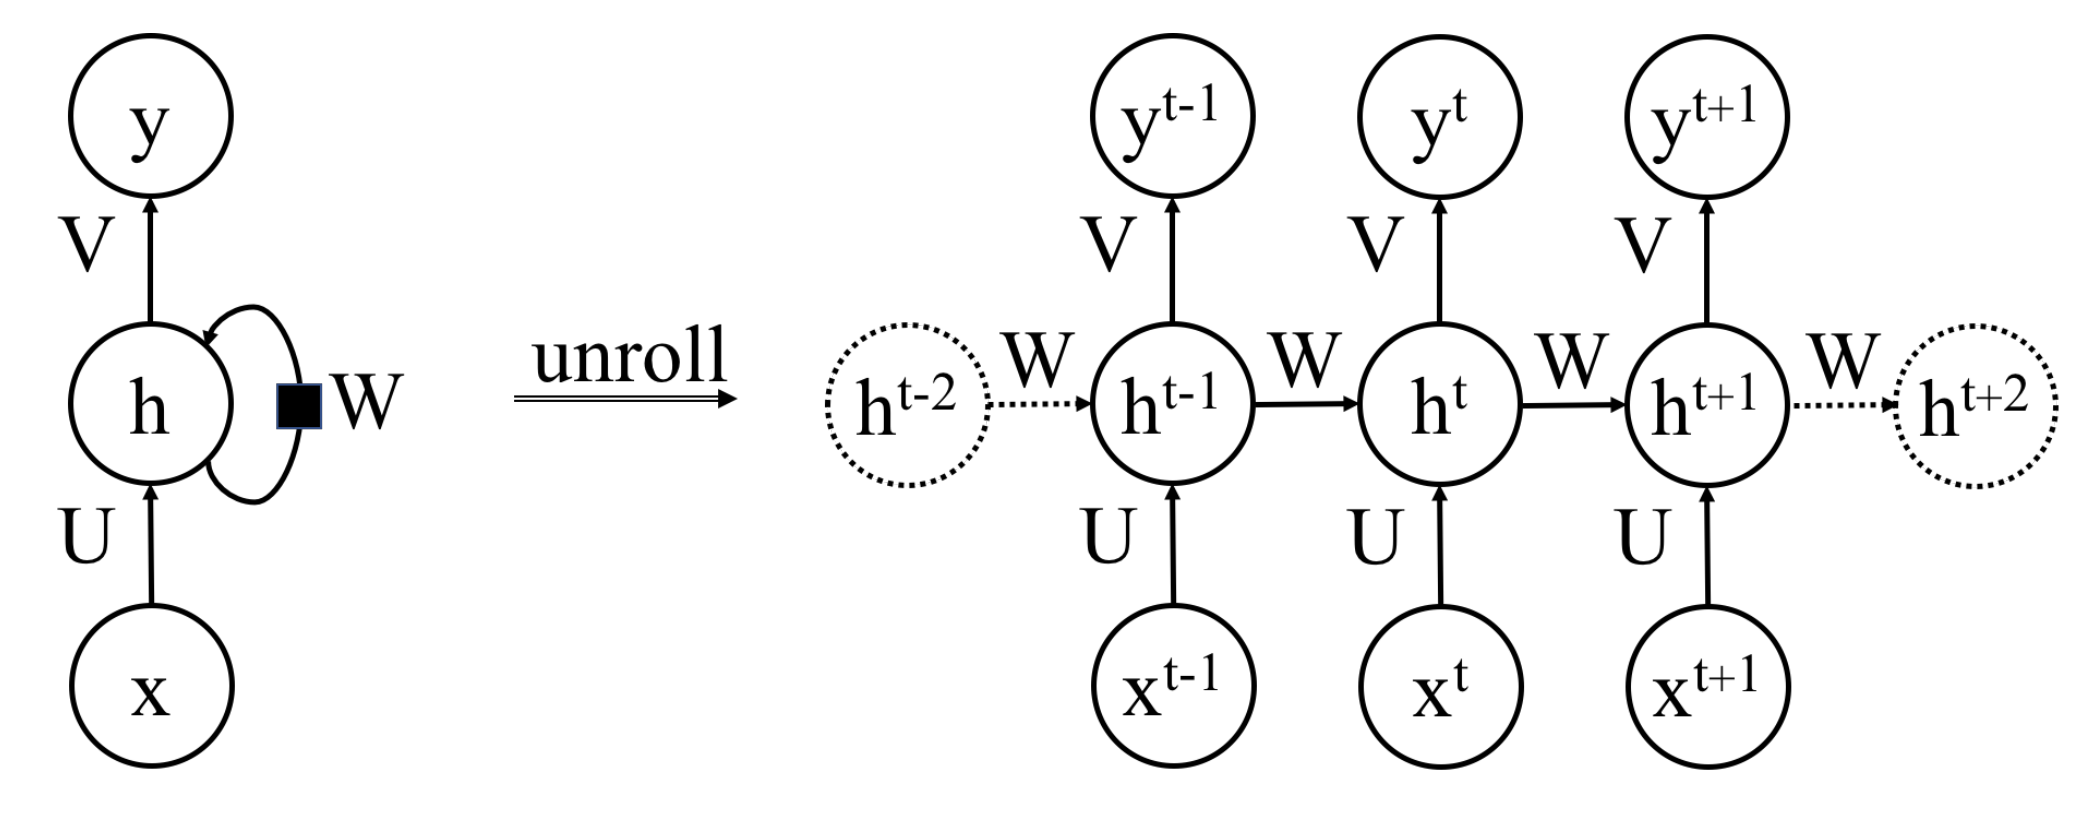
\includegraphics[width=0.9\linewidth]{rnn_unrolled.png}
\\Hidden state can be thought of as a noisy memory, compresses relevant aspects of sequence: $(\mathbf x^1,...,\mathbf x^{t-1})\mapsto \mathbf h^t$ (conceptually)\\
 For any fixed length $s$, the unrolled recurrent net corresponds to a feedforward net with $s$ hidden layers. Difference to MLP: sharing of parameters and inputs processed sequentially..\\
\textbf{Backpropagation (through time :P)}: sum over time steps\\
With $\dot\sigma_i^t:=\sigma'(\bar F_i(h^{t-1},x^t))$:\\
$\frac{\partial\mathcal R}{\partial w_{ij}}=\sum_{t=1}^s\frac{\partial\mathcal R}{\partial h_i^t}\cdot\frac{\partial h_i^t}{\partial w_{ij}}=\sum_{t=1}^s\frac{\partial\mathcal R}{\partial h_i^t}\cdot\dot\sigma_i^t\cdot h_j^{t-1}$\\
$\frac{\partial\mathcal R}{\partial u_{ik}}=\sum_{t=1}^s\frac{\partial\mathcal R}{\partial h_i^t}\cdot\frac{\partial h_i^t}{\partial u_{ik}}=\sum_{t=1}^s\frac{\partial\mathcal R}{\partial h_i^t}\cdot\dot\sigma_i^t\cdot x_k^{t}$\\
Example with setting: $y_{1:T}$ ground-truth outputs and $\hat y_{1:T}$ predictions, $a_t=F(x_t,h_{t-1},y_{t-1};\theta)$, $h_t=\sigma(a_t)$, $\hat y_t=G(h_t,\phi)$, $L_t=H(y_t,\hat y_t)$, $L=\sum_{t=1}^TL_t$. Derivative of $L$ wrt $\theta$:\\
$\frac{\partial L}{\partial \theta}=\sum_{t=1}^T\frac{\partial L_t}{\partial \hat y_t}\frac{\partial \hat y_t}{\partial h_t}\sum_{i=0}^t(\prod_{j=t}^{i+1}\frac{\partial h_j}{\partial a_j}\frac{\partial a_j}{\partial h_{j-1}})\frac{\partial h_i}{\partial a_i}\frac{\partial a_i}{\partial\theta}$\\
\textbf{Exploding/Vanishing gradients}: let  output in last step $\mathbf y=\mathbf y^s$\\
Then $\nabla_{\mathbf x^t}\mathcal R=[\prod_{r=t+1}^s\mathbf W^T\mathbf{S}(\mathbf h^r)]\cdot\mathbf J_H\cdot\nabla_\mathbf y\mathcal R, \quad \mathbf{S}(\mathbf h^r)=\text{diag}(\dot\sigma_1^r,...,\dot\sigma_n^r)$\\
Take spectral norm, and use $||\mathbf{AB}||_2\leq||\mathbf A||_2\cdot||\mathbf B||_2$. If $\sigma_{\max}(\mathbf W)<1$:\\ $||\nabla_{\mathbf x^t}\mathcal R||\leq\sigma_{\max}(\mathbf W)^{s-t}\cdot||\mathbf \mathbf J_H\cdot\nabla_\mathbf y\mathcal R||\overset{(s-t)\rightarrow\infty}{\rightarrow}0$\\
Conversely may explode if $\sigma_{\max}(\mathbf W)>1$\\
\textbf{Bi-directional network}: reverse order $\mathbf g^t=G(\mathbf x^t,\mathbf g^{t+1};\pmb\theta)$\\
Interweave the two hidden state sequences\\
\textbf{Deep recurrent network:} hierarchical hidden states of $l$ layers\\
$\mathbf h^{t,1}=F(\mathbf h^{t-1,1},\mathbf x^t;\pmb\theta)$\\
$\mathbf h^{t,l}=F(\mathbf h^{t-1,l},\mathbf h^{t,l-1};\pmb\theta), \quad l=2,...,L$
\subsection*{Memory Units}
\textit{Addressing the problem of vanishing/exploding gradients}\\
Gated units to learn long-term dependencies\\
Difficult to understand what units learn, resource-hungry and slow in learning\\
\textbf{LSTM}\\
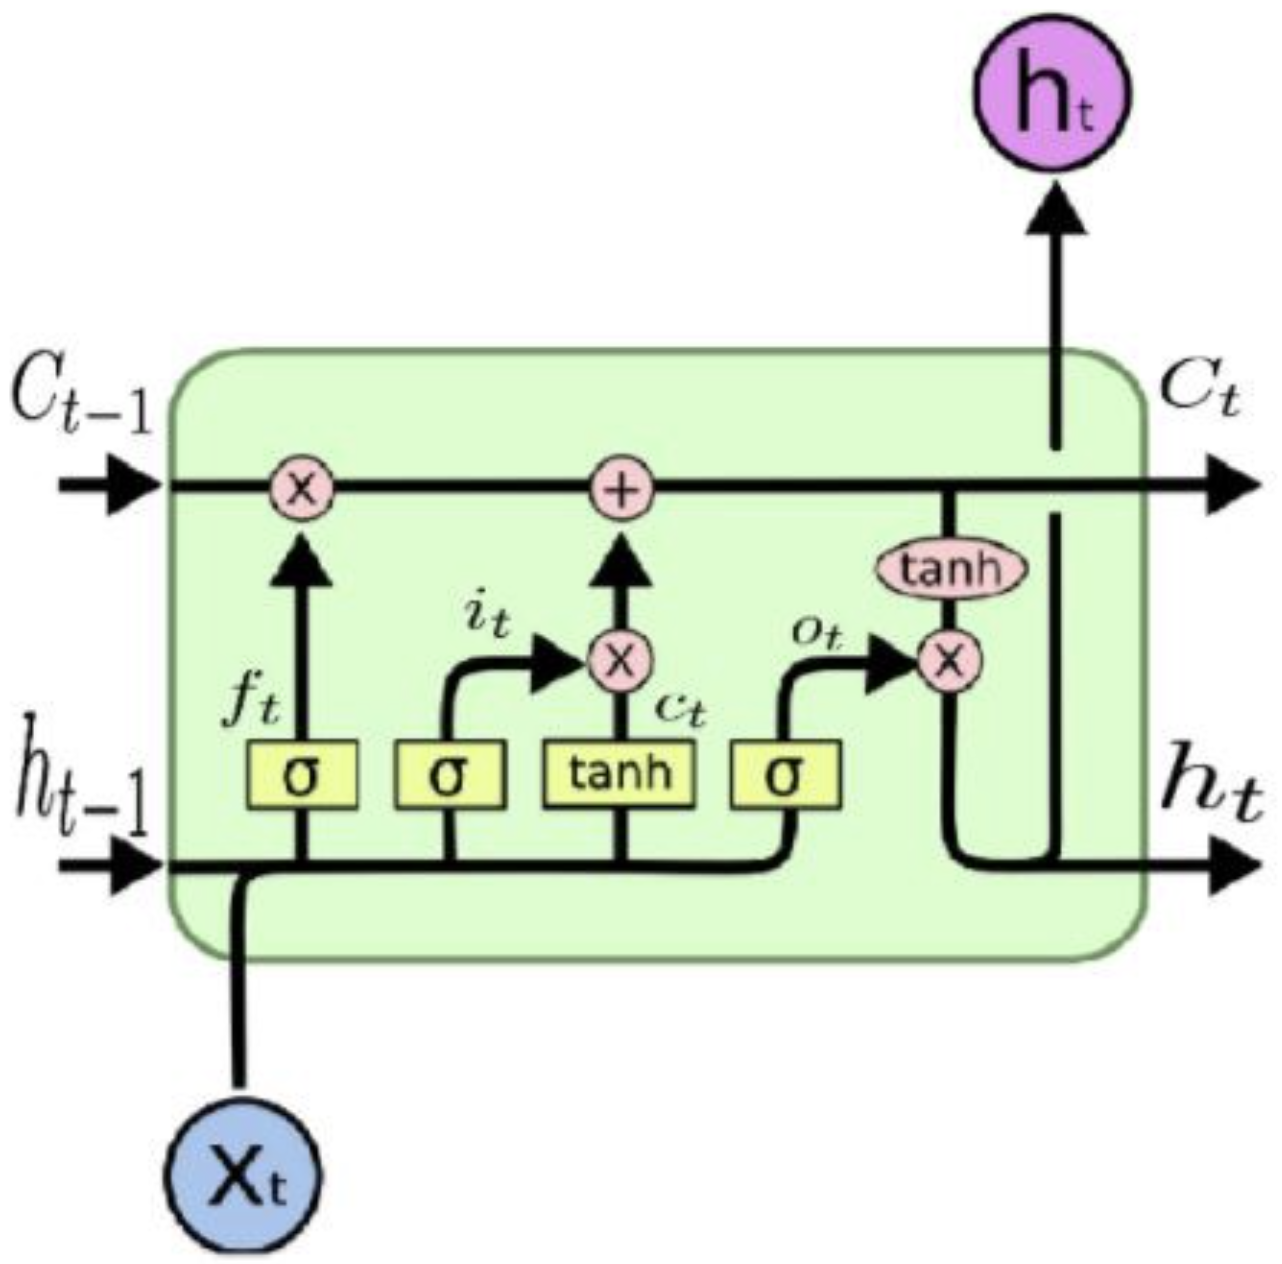
\includegraphics[scale=0.17]{lstm_cell.png}
\\Content $C$ has similar effect as ResNet for vanishing gradients\\
Forget gate: $f_t=\sigma(W_f\cdot[h_{t-1},x_t]+b_f)$\\
Input to memory: \\ $i_t=\sigma(W_i\cdot[h_{t-1},x_t]+b_i), \quad $
$\tilde C_t=\tanh (W_C\cdot[h_{t-1},x_t]+b_C)$\\
Updating memory: $C_t=f_t*C_{t-1}+i_t*\tilde C_t$\\
Output gate:\\
$o_t=\sigma(W_o[h_{t-1},x_t]+b_o), \quad h_t=o_t*\tanh (C_t)$\\
Gates: input gate, output gate and forget gate\\
\textbf{Gated Recurrent Unit (GRU)}\\
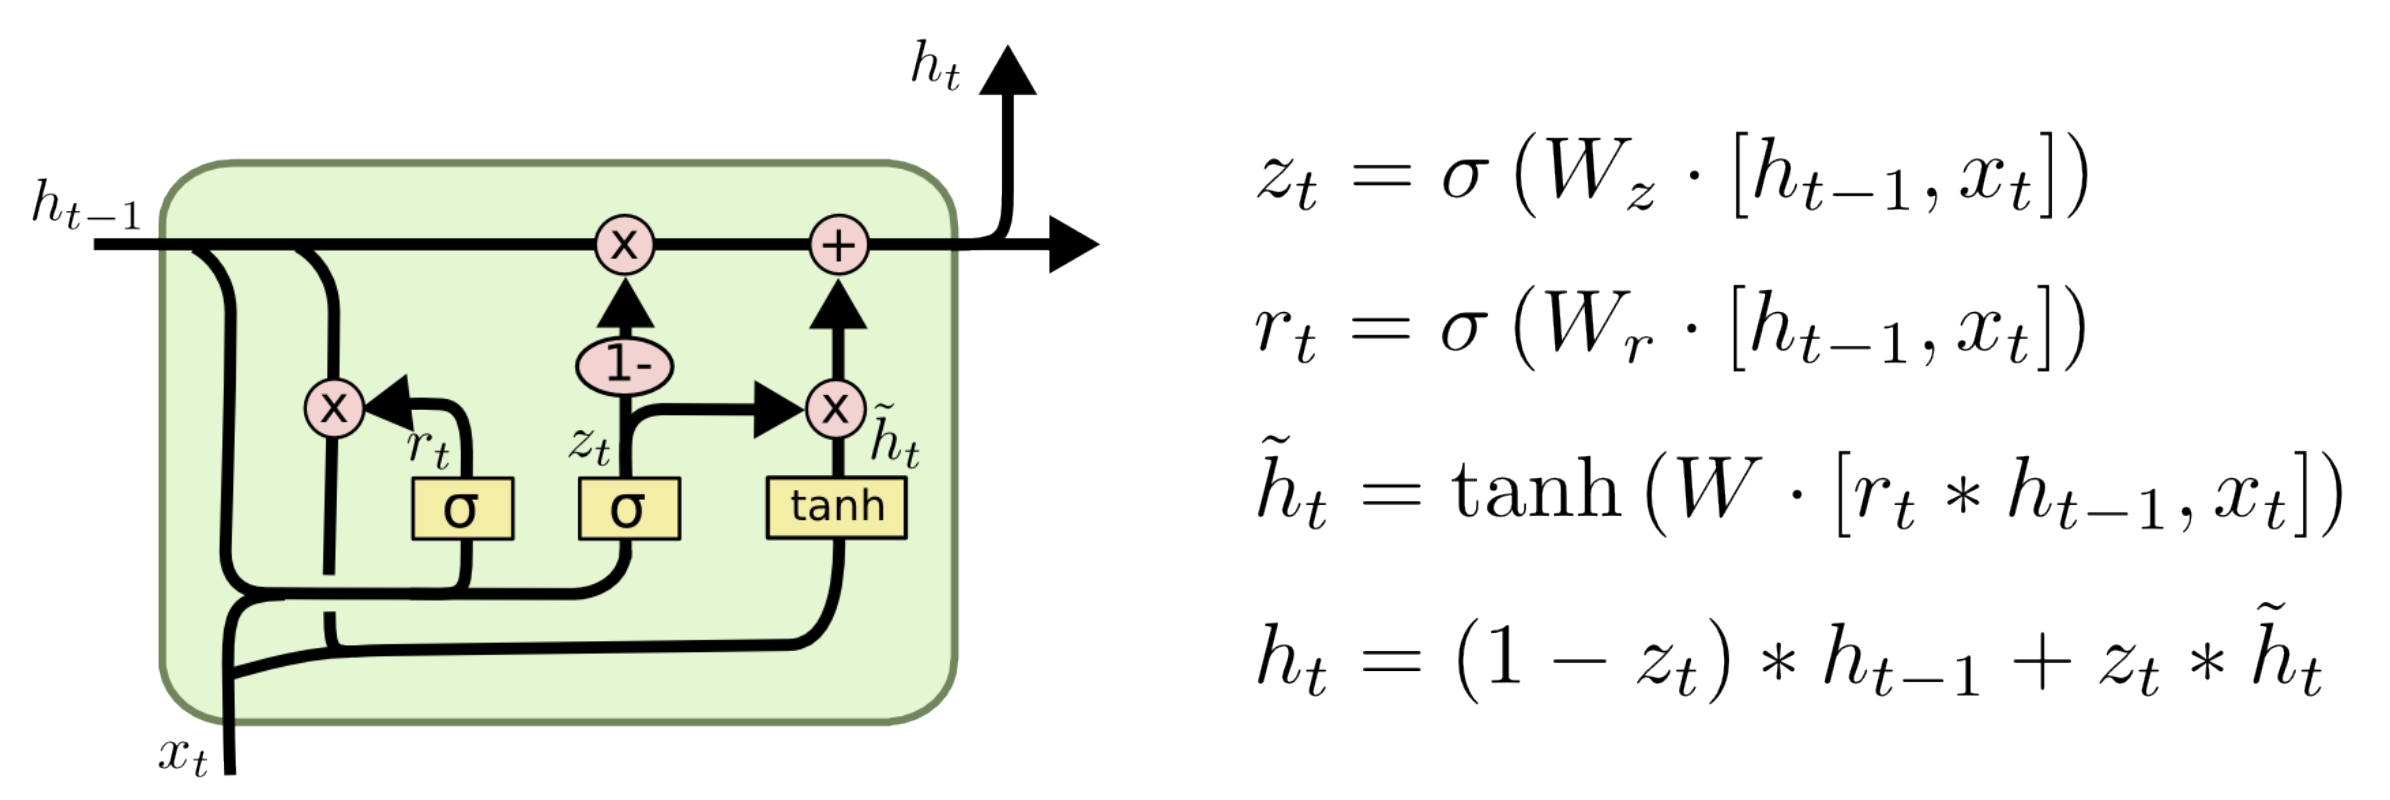
\includegraphics[scale=0.17]{gru.png}\\
Gates: update gate and reset gate \\
Here $h$ is both state and content, computed as a convex combination of old and new information
\subsection*{Learning sequences - Seq2Seq}
Goal: learn $p(\mathbf y^{1:T}|\mathbf x^{1:T})\approx \prod_{t=1}^Tp(\mathbf y^t|\mathbf x^{1:t},\mathbf y^{1:t-1})$\\
Naive implementation: $p(\mathbf y^t)$ depends on $\mathbf y^{1:t-1}$ only through $\mathbf h^t$\\
$\Rightarrow$ remedy by feeding back previous outputs!\\
\textbf{Teacher forcing:} When training, compute loss on predicted output but feed back in correct output. During prediction feed back predicted outputs. Improves learning BUT gives exposure bias\\
\textbf{Encoder-Decoder model}: \\
Encoder: $(\mathbf x^1,...,\mathbf x^T)\mapsto \mathbf z, \quad \mathbf z=\mathbf h^T$ (RNN)\\
Decoder $\mathbf z\mapsto (\mathbf y^1,...,\mathbf y^S)$ (RNN with output feedback)\\
Can also be used for image captioning with CNN encoder
\section*{Attention} 
\textit{Instead of compressing the whole sequence into a vector, determine where to look}
\subsection*{Self attention}
\textbf{Gating function:} Given query $\pmb\xi\in\mathrm R^n$ and values $\mathbf x^t\in\mathrm R^m$, \\$f_\phi(\pmb\xi, (\mathbf x^1,...,\mathbf x^s))=\frac{1}{\sum_j \exp[\phi(\pmb\xi,\mathbf x^j)]}\begin{bmatrix} \exp[\phi(\pmb\xi,\mathbf x^1)] \\...\\ \exp[\phi(\pmb\xi,\mathbf x^s)] \end{bmatrix}$\\
Simplest choice for similarity function when $m=n$: $\phi(\pmb\xi,\mathbf x)=\pmb\xi\cdot\mathbf x$\\
\textbf{Transfer function:} $F(\pmb\xi, (\mathbf x^1,...,\mathbf x^s))=[\mathbf x^1 \quad ... \quad \mathbf x^s]\cdot f_\phi(\pmb\xi, (\mathbf x^1,...,\mathbf x^s))$\\
i.e. computes convex combination of inputs wrt attention weights\\
\textbf{RNN with attention (Seq2Seq):} combining ideas of encoding information relevant for the future (RNNs) and selecting what is relevant in retrospective (attention)\\
Attend to hidden state sequence $(\mathbf h_e^1,...,\mathbf h_e^s)$ of encoder with query $\pmb\xi^i$ produced as hidden states by decoder. Use this as input into decoder, which produces hidden states $(\pmb\xi^1,...,\pmb\xi^t)$ and output sequence $(\mathbf y^1,...,\mathbf y^t)$ 
%Happens during decoding. For each word in sentence, assign weights to words from input sentence.\\
\subsection*{Memory Networks}
Recurrent attention model over possibly large external memory\\
\textbf{Recursive associative recall:} Given query $\mathbf q$ (e.g. question), find best matching memory cell $i$, use its content $\mathbf m_i$ and $\mathbf x$ to generate new query - repeat
\subsection*{Transformers}
\textit{Attention is all you need}\\
\textbf{Key-Value attention map:} given KV pairs $(\mathbf x^i,\mathbf z^i)$,\\ $F(\pmb\xi,((\mathbf x^1,\mathbf z^1),...,(\mathbf x^s,\mathbf z^s)))=[\mathbf z^1\quad...\quad\mathbf z^s]\cdot f(\pmb\xi,(\mathbf x^1,...,\mathbf x^s))$\\
$\Rightarrow$ keys determine where to look, values what features to extract\\
Similarity function: $\phi(\pmb\xi,\mathbf x)=\frac{\pmb\xi\cdot\mathbf x}{\sqrt n},\quad \pmb\xi,\mathbf x\in\mathrm R^n$\\
Assuming entries sampled from standard Gaussian, this gives standard scaling. Good since softmax can be sensitive to large input values (which kills gradient and slows down learning)\\
\textbf{Multi-headed attention:} $G(\pmb\xi,(\mathbf x^t,\mathbf z^t)_{t=1}^s)=\mathbf W\begin{bmatrix}F_1(\pmb\xi,(\mathbf x^t,\mathbf z^t))\\...\\F_h(\pmb\xi,(\mathbf x^t,\mathbf z^t)) \end{bmatrix}$\\
$F_j(\pmb\xi,(\mathbf x^t,\mathbf z^t))=F(\mathbf W_j^q\pmb\xi,(\mathbf W_j^x\mathbf x^t,\mathbf W_j^z\mathbf z^t))$\\
Alt.: $\mathbf Y=\text{softmax}(\mathbf{XW}_q\mathbf W_k^T\mathbf X^T)\mathbf{XW}_v, \mathbf W_{\{q,k,v\}}\in\mathrm R^{d\times hd},\mathbf{X,Y}\in\mathrm R^{L\times d}$\\
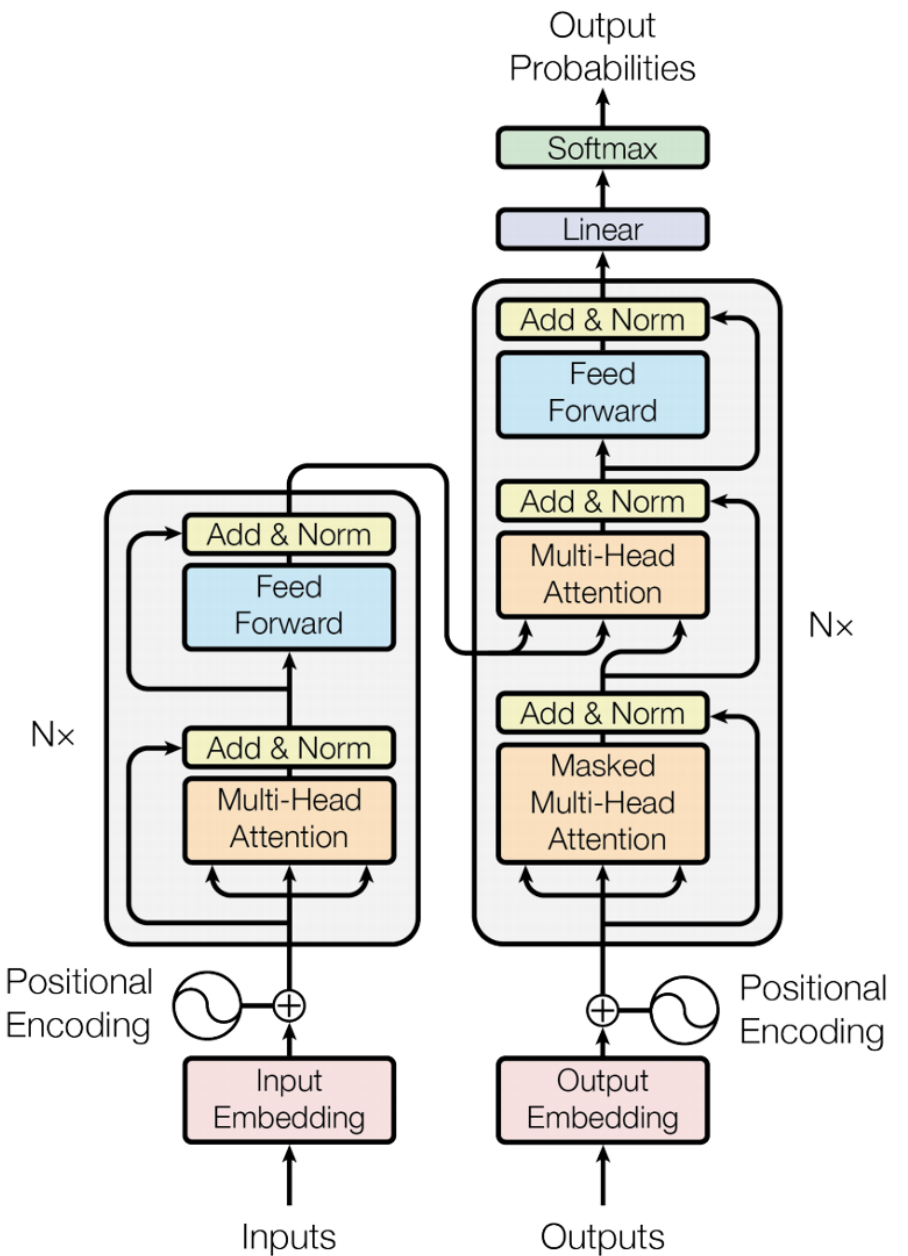
\includegraphics[scale=0.25]{transformer.png}\\
\textbf{1. Input embedding} Accounts for meaning\\
\textbf{2. Positional Encodings} Accounts for position in the input sentence. Normally use sinusoidal functions. For position $t$ and feature $k$:\\ $p_{tk}=\begin{cases} \sin(t\omega_k) \quad k \text{ even} \\ \cos(t\omega_k) \quad k \text{ odd} \end{cases} \omega_k=C^{k/n}, C=10000$\\
\textbf{3. Creating Masks} In decoder, to prevent peaking ahead.\\
\textbf{4. Multi-Head Attention Layer} Split embedding into $N$ heads and perform attention on each. Three types: Self, masked and mixed.\\
\textbf{5. Feed-Forward layer}
\subsection*{Applications in NLP}
\textit{Construct word embeddings that reflect the context}\\
\textbf{ELMo}: Input fixed embeddings on character level, build word representations with CNNs, then stack left-to-right LSTM and right-to-left LSTM. Output (for each word) is convex combination of hidden states over layers. Out-of-vocabulary (not restricted to fixed vocabulary). Train in task-specific manner.\\
\textbf{BERT}: Input sub-word unit embeddings. Leverage attention - take query and retrieve keys \& values from words in context. Insight: do not need to learn a language model. Train by word masking task - predict missing word in text. Also do next sentence prediction in pre-training. Can fine-tune for specific downstream task. \textbf{BERTology} -  representations hierarchical, struggles with negation, incomplete syntactic knowledge etc\\
\textbf{GPT-n}: Few, one or zero shot learning - add task description \& examples to working memory and let model do the rest.
\section*{Theory of DNNs}
\subsection*{VC Theory}
\textbf{Shattering coefficient: }maximum number of ways in which $n$ points can be classified by function class $\mathcal F$ \\
$\Rightarrow \mathcal S_{\mathcal F}(n)=\sup_{(\mathbf x_1,...,\mathbf x_n)}|\{(f(\mathbf x_1),...,f(\mathbf x_n)): f\in\mathcal F\}|\leq 2^n$\\
Say that $\mathcal F$ \textbf{shatters} a set of $n$ points if $S_\mathcal F(n)=2^n$\\
\textbf{VC-dim} The VC-dim of $\mathcal{F}$ is $n$ $\iff$ there is a set of size $n$ that is shattered by $\mathcal{F}$, and \textbf{no} set of size $n+1$ is shattered by $\mathcal{F}$. \\ $\text{VC-dim}(\mathcal{F}) \leq  \log_2(|\mathcal{F}|)$\\
\textbf{Vapnik-Chervonenkis Theorem:} For any $\delta>0$, with probability at least $1-\delta$:\\
$\forall f\in\mathcal F, \quad \mathcal R(f)\leq\mathcal R_n(f)+2\sqrt{2\cdot\frac{\log\mathcal S_\mathcal F(2n)+\log\frac{2}{\delta}}{n}}$
\subsection*{PAC Bayes Bounds}
\textbf{Donsker's Theorem:} For any $P>>Q$, $P$-measurable function $\phi$ \\ $\mathrm E_Q[\phi]\leq \text{KL}(Q||P)+\log\mathbb E_P[e^\phi]$\\
\textbf{McAllister theorem} $\forall$ fixed $P$ and any $Q$, $\epsilon \in (0,1)$ w.prob $ \geq \epsilon$ over sample set $S$: 
$\mathbb{E}_Q[e_f] - \mathbb{E}_Q[e_f^S] \leq \sqrt{\frac{2}{|S|}\left[KL(Q||P) + \ln\left( \frac{2\sqrt{|S|}}{\epsilon}\right)\right]}$. \\
\textbf{Interpretation for DNNs:} Take $P=\mathcal N(\theta_0,\lambda\mathrm I)$ to be prior over parameter space. $Q=\mathcal N(\theta,\text{diag}(\sigma^2))$ (learned from data) is a distribution over $\mathcal F$, where our function $f$ is sampled from. Minimize bound together with (surrogate of) empirical risk.\\
A \textbf{stochastic neural network} is a network whose weights are drawn from a distribution $Q$ each time data is propagated through the network.
\section*{Learning on Graphs}
\textbf{Motivation}: Data may not be sampled iid but could be graph-structured\\
\textbf{Use-cases}: Node classification, link prediction, generative modeling\\
\textbf{Focus here}: GCN from paper \textit{Semi-Supervised Classification with Graph Convolutional Networks}, Kipf \& Welling 2017\\
\textbf{Idea}: To make prediction on node, gather information from context in graph\\
Let $\mathbf X\in\mathbb R^{d\times n}$ be graph of $n$ nodes with $d$ features, then define:\\
$\mathbf X^{l+1}=\sigma(\mathbf W^l\mathbf X^l \mathbf Q),\quad $where $\mathbf{WX}$ sums over dimensions and $\mathbf{XQ}$ sums over data points / nodes (to learn from neighborhood)\\
Define degree-normalized matrix $Q=\tilde D^{-\frac{1}{2}}\tilde A\tilde D^{-\frac{1}{2}}$, where $\tilde D$ is the diagonal degree matrix of $\tilde A:=A+\mathrm I_n$ and $A$ is adjacency matrix. It holds that:\\
$q_{ij}=\frac{a_{ij}+\delta_{ij}}{\sqrt{\tilde d_{i}\tilde d_j}}, \quad \tilde d_i=1+\sum_j A_{ij}, \quad \delta_{ij}=\begin{cases} 1, \quad i=j \\ 0, \quad i\neq j\end{cases}$\\
Activations from neighbors are mixed together with respective $Q$-weights: and $(X^lQ)_{ij}=([x^l[1],...,x^l[n]]\cdot Q)_{ij}=\sum_{k=1}^nx_{ik}q_{kj}$\\
$\Rightarrow (X^lQ)_{\bullet j}=\sum_{k}q_{kj}\cdot x^l[k]\quad$ (sum over neighborhood of node $j$)\\
\textbf{Cyclic chain:} For regular lattice graph, $Q$ is Toeplitz matrix and thus related to convolutional layer with window size same as neighborhood size\\
\textbf{Linear Shift Invariant Filter:} linear function $H$ over graph with adjacency matrix $A$ such that $H(Ax)=A(Hx)$. $H$ is $A$-shift invariant iff: $\quad H=\theta_0\mathrm I+\theta_1A+...+\theta_nA^n$\\
If we consider $H(\theta_0,\theta_1)=\theta_0\mathrm I+\theta_1(D^{-\frac{1}{2}}AD^{-\frac{1}{2}})$ and $\theta_0=\theta_1$ then largest eigenvalue is $2$, which can be a source of instabilities. Motivates $\mathrm I + D^{-\frac{1}{2}}AD^{-\frac{1}{2}}\mapsto \tilde D^{-\frac{1}{2}}\tilde A\tilde D^{-\frac{1}{2}}$, which has largest EV $1$ 
\section*{Adversarial Robustness}
\textit{Adversarial examples are small manipulations of input which cause the model to change its prediction}\\
\textbf{Additive adversarial manipulation}: Find $x\in\mathrm R^d$ s.t. $k(x+r)\neq k(x)$ and $x+r$ similar to $x$. As proxy for \textit{similar}, use $l_p$-norm robustness - $||r||_p$ should be small\\
Two approaches to measure robustness to adversarial perturbations: unconstrained \& constrained perturbations
\subsection*{Unconstrained Perturbations - DeepFool}
\textit{Find smallest perturbation in $l_p$-norm that induces mistake}\\
Let $f:\mathrm R^d\rightarrow \mathrm R^C$ be the logits, i.e. outputs before softmax, and wlog $k(x)=1$\\
Disadvantage of approach: Typically get close to decision boundary which may be exploited to detect them (can e.g. train a classifier to detect them given some confidence threshold)\\
$\hat\rho_{\text{adv}}=\frac{1}{n}\sum_{i=1}^n\frac{||r(x_i)||_2}{||x_i||_2}$\\
\textbf{DeepFool - Binary case:} $\arg\underset{r}{\min} ||r||_p$ s.t. $f_2(x+r) - f_1(x+r)>0$\\
First-order Taylor approximation around $x$, rewrite constraint:\\ $(\nabla_x f_1(x)-\nabla_x f_2(x))^Tr+f_1(x)-f_2(x)<0 \Rightarrow$ linearized classifier\\
Solve iteratively until $k(x+r_1+...+r_n)\neq k(x)$\\
Optimum in each step, $1/p+1/p^*=1$: \\ $r^*=\frac{f_1(x)-f_2(x)}{||\nabla_xf_1(x)-\nabla_xf_2(x)||^{p^*}_{p^*}}\cdot|\nabla_xf_1(x)-\nabla_xf_2(x)|^{p^*-1}\odot\text{sgn}(\nabla_xf_1(x)-\nabla_xf_2(x))$\\
\textbf{DeepFool - General case:} Optimize wrt $r_i$ for each class and update in the direction of smallest $r_i$\\
$x_0=x$\\
$x_k=x_{k-1}+\underset{j\neq k(x)}{\min}\{\frac{|h_j(x_{k-1})|}{||\nabla_xh_j(x_{k-1})||^{p^*}_{p^*}}\cdot |\nabla_xh_j(x_{k-1})|^{p^*-1}\odot\text{sgn}(\nabla_xh_j(x_{k-1}))\}$, where $h_j(x_{k-1})=f_j(x_{k-1})-f_{k(x)}(x_{k-1})$
\subsection*{Constrained Perturbations - PGD}
\textit{Given $\epsilon>0$ find perturbation $r$ with $||r||_p\leq\epsilon$}\\
Disadvantage of approach: Perturbation found can be larger than the minimal one within ball\\
\textbf{Projected Gradient Descent / Ascent}:\\
$x_0\sim\mathcal U(\mathcal B_\epsilon^p(x))$\\
$x_k=\Pi_{\mathcal B_\epsilon^p(x)}(x_{k-1}+\alpha\underset{v_k: ||v_k||_p\leq 1}{\arg\max}v_k^T\nabla_xl(y,f(x_{k-1})))$\\
where $r_k=x_k-x, \quad\Pi_{\mathcal B_\epsilon^p(x)}(\tilde x)=\arg\min_{x^*\in \mathcal B_\epsilon^p(x)}||\tilde x-x^*||_2$ and $v^*=\underset{v: ||v||_p\leq 1}{\arg\max}v^Tz=\frac{\text{sign}(z)\odot|z|^{p^*-1}}{||z^*||^{p^*-1}_{p^*}}$\\
\textbf{Adversarial Training:} Most effective method for improving robustness. Can combine with e.g. PGD:\\
$\underset{\theta}{\min}\underset{||r||_p\leq \epsilon}{\max}(f_{\theta^t}(x+r),y)$\\
Accuracy on clean data degrades $\rightarrow$ more data \\
Network overfits to attacks used in training $\rightarrow$ use many iterations for PGD\\
Takes longer to train $\rightarrow$ explicit regularization\\
Mode of failure 1: gradient wrt input norm becomes too small \\
Mode of failure 2: gradient wrt input becomes noisy $\rightarrow$ not find closest perturbation
\subsection*{Benefits beyond robustness and security}
\textbf{Interpretability} - robust networks learn more human-interpretable features \\
\textbf{Transfer learning} - robust networks generalize better across domains \\
\textbf{Generative modeling} - robust networks perform better in generative tasks 
\subsection*{Adversarial training and operator norm regularization}
Linearization: $f(\mathbf x+\Delta\mathbf x)\approx f(\mathbf x)+J_f(\mathbf x)\Delta\mathbf x$\\
$\Rightarrow \frac{||f(\mathbf x+\Delta\mathbf x)-f(\mathbf x)||_2}{||\Delta\mathbf x||_2}\approx\frac{||J_f(\mathbf x)\Delta\mathbf x||_2}{||\Delta\mathbf x||}\leq \sigma(J_f(\mathbf x))=:\underset{v:||v||_2\leq 1}{\max}||J_f(\mathbf x)v||_2$\\
So from a robustness perspective, want small operator norm\\
\textbf{Data-independent spectral norm reg.:} $\sigma(J_f(\mathbf x))\leq\prod_{l=1}^L\sigma(\mathbf W^l)$\\
Generalizes from train to test set but can be arbitrarily loose\\
\textbf{Data-dependent:} $\min_\theta\mathrm E_{(\mathbf x,\mathbf y)\sim\tilde P}[l(y,f(\mathbf x))+ \frac{\tilde\lambda}{2}\sigma(J_f(\mathbf x))^2]$,\\ where $\sigma(J_f(\mathbf x))$ is computed by the power method\\
$l_p$-norm constrained PGA based adversarial training with an $l_q$-norm loss on the logits of clean and perturbed inputs is equivalent to data-dependent $(p, q)$ operator norm regularization.
\section*{VAEs}
\subsection*{Linear Factor Analysis}
Latent variable prior $\mathbf z\sim\mathcal N(\mathbf 0,\mathrm I), \quad \mathbf z\in\mathrm R^m$\\
Linear observation model for $\mathbf x\in\mathrm R^n: \quad\mathbf x=\pmb\mu+\mathbf{Wz}+\pmb\eta, \\ \pmb\eta\sim\mathcal N(\mathbf 0, \pmb\Sigma),\quad \pmb\Sigma:=\text{diag}(\sigma_1^2,...,\sigma_n^2)$\\
Can be shown that: $\mathbf x\sim\mathcal N(\pmb\mu,\mathbf{WW}^T+\pmb\Sigma)$\\
Non-identifiability, for orthogonal $\mathbf Q$: $(\mathbf{WQ})(\mathbf{WQ})^T=\mathbf{WW}^T$\\
Posterior inference:\\ $\pmb\mu_{\mathbf{z|x}}=\mathbf W^T(\mathbf{WW}^T+\pmb\Sigma)^{-1}(\mathbf x-\pmb\mu)$\\
$\pmb\Sigma_{\mathbf{z|x}}=\mathbf I-\mathbf W^T(\mathbf{WW}^T+\pmb\Sigma)^{-1}\mathbf W$\\
MLE: $\pmb\theta=(\pmb\mu,\mathbf W)\overset{\max}{\leftarrow}\log p(\mathbf X;\pmb\mu,\mathbf W)$, has no closed form solution\\
\textbf{Probabilistic PCA}: when $\pmb\Sigma=\sigma^2\mathbf I$
\subsection*{Variational Autoencoders}
\textit{Generalize factor analysis with depth}\\
Noise variable: $\quad \mathbf z\sim\mathcal N(\mathbf 0, \mathbf I)$\\
Density unavailable explicitly, so can't do MLE:\\ $\pmb\theta\overset{\max}{\leftarrow}\sum_{i=1}^n\log p(\mathbf x[i];\pmb\theta)$\\
Max. ELBO: $\log p(\mathbf x;\pmb\theta)\geq \mathrm E_{\mathbf z\sim q(\mathbf z;\mathbf x)}[\log p(\mathbf x|\mathbf z;\pmb\theta)]-\text{KL}(q(\mathbf z;\mathbf x)||p(\mathbf z))$\\
Can think of $q(\mathbf z;\mathbf x)$ as posterior ($=p(\mathbf{z|x})$), restricted to (typically Gaussian) variational family: \\ $\mathcal N(\pmb\mu(\mathbf x),\pmb\Sigma(\mathbf x)), \quad \pmb\Sigma(\mathbf x)=\text{diag}(\sigma_1^2(\mathbf x),...,\sigma_n^2(\mathbf x))$ (output of encoder)\\
Optimizing over $q$ involves gradients of expectations $\Rightarrow$ stochastic backpropagation / re-parameterization trick:\\
$\mathbf z\sim\mathcal N(\pmb\mu,\pmb\Sigma) \quad \Leftrightarrow \quad\mathbf z=\pmb\mu+\pmb\Sigma^{1/2}\pmb\eta, \quad \pmb\eta\sim\mathcal N(\mathbf 0,\mathrm I)$\\
$\Rightarrow$ can now backpropagate wrt $\pmb\mu$ and $\pmb\Sigma^{1/2}$!
\section*{Generative Models}
\subsection*{Density Estimation}
\textit{Learn a parametrized model $p_\theta(\mathbf x)$ to be indistinguishable from true generative process $p(\mathbf x)$}\\
\textbf{1 - Prescribed model}: Density explicitly specified (and accessible). Can do MLE. Challenge: Normalizing model\\
\textbf{2 - Implicit model}: Transformation of densities, can describe density through integration by substitution\\
\textbf{Integration by substitution - change of variables formula}:\\ $\mathbf x=F(\mathbf z), \quad p_X(\mathbf x)=p_Z(F^{-1}(\mathbf x))|\text{det}(\partial F)|^{-1}$, $p_X$ pushforward of $p_Z$
\subsection*{Normalizing Flows}
Bijections $F$ which are convenient to compute, invert and calculate $|\text{det}(\partial F)|$\\
$F=F_L\circ\cdot\cdot\cdot\circ F_1, \quad F^{-1}=F^{-1}_1\circ\cdot\cdot\cdot\circ F_L{-1}$\\
$\Rightarrow \text{det}(\partial F)=\prod_{l=L}^1\text{det}(\partial F_l\circ F_{l-1:1}), \quad \text{det}(\partial F^{-1})=\text{det}(\partial F)^{-1}$\\
Log-likelihood: $\log p(\mathbf x | \mathbf z)=-\sum_{l=1}^L\log |\text{det}(\partial F_l\circ F_{1:l-1})|$\\
\textbf{Linear flow}: $F(\mathbf x)=\mathbf{Az+b} \Rightarrow \mathcal O(n^3)$ to compute determinant and inverse. If $A$ diagonal, simple \& efficient but not powerful.\\
If $A$ triagonal: $\text{det}(A)=\prod_i A_{ii},\quad$ but $A^{-1}$ expensive...\\
\textbf{Invertible linear time flows}: $F(\mathbf z)=\mathbf z+\mathbf u\sigma(\mathbf{w\cdot z}+b)$ \\
Determinant: $|\text{det}(\partial F)|=|1+\sigma'\mathbf u^T\mathbf w|$\\
In general, normalizing flows not powerful enough as Jacobian condition is too restrictive $\Rightarrow$ Likelihood-free methods
\subsection*{Generative Adversarial Networks (GANs)}
\textit{Derive training signal for generator $G$ from classifier $D$ that discriminates data from model-generated samples}\\
For sample $\mathbf x$ and model label $y$: $\tilde p_\theta(\mathbf x, y)=\frac{1}{2}(yp(\mathbf x)+(1-y)p_\theta(\mathbf x))$\\
$\Rightarrow$ balanced binary classification problem\\
\textbf{Optimal discriminator - Bayes optimal classifier}: \\$q_\theta(\mathbf x)=\frac{p(\mathbf x)}{p(\mathbf x)+p_\theta(\mathbf x)}=\mathrm P(y=1|\mathbf x)$\\
Train generator by minimizing log-likelihood (=JS for BOC)\\ $l^*(\theta):=\mathrm E_{\tilde p_\theta}[y\log q_\theta(\mathbf x)+(1-y)\log(1-q_\theta(\mathbf x))]=...=\text{JS}(p,p_\theta)-\log 2$\\
Bayes optimal classifier not accessible, define classification model: $q_\phi: \mathbf x\mapsto [0,1], \quad \phi\in\Phi$\\
It holds that: $l^*(\theta)\geq\sup_{\phi\in\Phi}l(\theta,\phi)\quad$ (given a generator, the log-likelihood with the BOC is an upper bound for the log-likelihood with any other classifier)\\
\textbf{General objective}: $l(\theta,\phi):=\mathrm E_{\tilde p_\theta}[y\log q_\phi(\mathbf x)+(1-y)\log(1-q_\phi(\mathbf x))]$\\
Saddle-point problem: $\theta^*:=\arg\min_{\theta\in\Theta}\{\sup_{\phi\in\Phi}l(\theta,\phi)\}$\\
Inner sup is impractical $\Rightarrow$ SGD heuristic: \\
$\theta^{t+1}=\theta^t-\eta\nabla_\theta l(\theta^t,\phi^t), \quad \phi^{t+1}=\phi^t+\eta\nabla_\phi l(\theta^{t+1},\phi^t)$\\
Alternatively, with $D(\cdot)$ the probability discriminator assigns that sample is from real data:\\ $\min_G\max_D\mathrm E_{\mathbf x\sim p(\mathbf x)}[\log D(\mathbf x)]+\mathrm E_{\mathbf z\sim p_\mathbf z(\mathbf z)}[\log(1-D(G(\mathbf z)))]$\\
\textbf{Mode collapse (Helvetica scenario)}: Generator collapses too many values of $z$ to similar values of $x$ and does not capture the diversity in $p(\mathbf x)$. Avoid by not training $G$ too much without updating $D$. Can lead to good-looking samples without diversity\\
\textbf{Vanishing gradient}: If the discriminator becomes too strong the gradient wrt the parameters of the generator vanishes ($\rightarrow 0$), so there will be no learning signal for the generator and it will not improve. Can lead to noisy/blurry samples but good variability\\
$\Rightarrow$ trade-off\\
\textbf{Why does minimizing Jensen-Shannon divergence work?}\\ Definition: $\text{JS}(Q||P)=\frac{1}{2}\text{KL}(P||\frac{P+Q}{2})+\frac{1}{2}\text{KL}(Q||\frac{P+Q}{2})$\\
In MLE we minimize the forward KL-divergence $\text{KL}(P||Q)=\int_xp(x)\log\frac{p(x)}{q(x)}dx$, which leads $q(x)$ to spread its mass over the whole support of $p(x)$, which is why samples from e.g. VAEs tend to be blurry. \\
If we minimize the reverse KL-divergence $\text{KL}(Q||P)$, $q(x)$ can be set to zero when $p(x)>0$, which leads to a $q(x)$ that focuses on certain mode(s) of $p(x)$. \\
Want something in between where whole support of $p(x)$ is covered while $q(x)=0$ where $p(x)=0$ $\Rightarrow$ \textbf{JS-divergence}!
\end{multicols*}
\end{document}